This chapter discusses the performance level of a single ipvs load balancer.
First the author evaluated the load balancer functionality using physical servers in on-premise data center and compared performance level with existing iptables DNAT and nginx as a load balancer within a 1Gbps network environment.
Then experiment was extended into the 10Gbps network environment to investigate the performance limitations of the proposed load balancer and a method to improve them.
Furthermore, the author also carried out the performance measurement in GCP and AWS to show that the containerized ipvs load balancer is runnable and has the same characteristics in the cloud environment.
The following sections explain these in further detail.

\section{On-premise experiment with 1Gbps Load balancer}
\subsection{Benchmark method}

A set of throughput measurement was carried out using an HTTP benchmark program, wrk\cite{Glozer2016}.
Figure~\ref{fig:benchmark-setup}(\subref{fig:benchmark-schem}) illustrates a schematic diagram of the experimental setup.
Multiple {\em pods} are deployed on multiple nodes in the Kubernetes cluster. 
In each {\em pod}, an nginx web server pod that returns the IP address of the {\em pod} are running.
The author set up the ipvs, iptables DNAT, and nginx load balancers on one of the nodes.
All the nodes and the benchmark client are connected to a 1Gbps network switch as in Figure~\ref{fig:benchmark-setup}(\subref{fig:bench_1g}).

The author measured the throughput, Request/sec, of the web service running on the Kubernetes cluster as follows:
The HTTP GET requests are sent out by the wrk on the client machine toward the nodes,
using destination IP addresses and port numbers that are chosen based on the type of the load balancer on which the measurement is performed.
The load balancer on the node then distributes the requests to the {\em pods}.
Each {\em pod} returns HTTP responses to the load balancer, after which the load balancer returns them to the client.
Based on the number of responses received by wrk on the client, 
load balancer performance, in terms of Request/sec can be obtained. 

\begin{figure}
\begin{subfigure}[t]{\columnwidth}
  \centering
  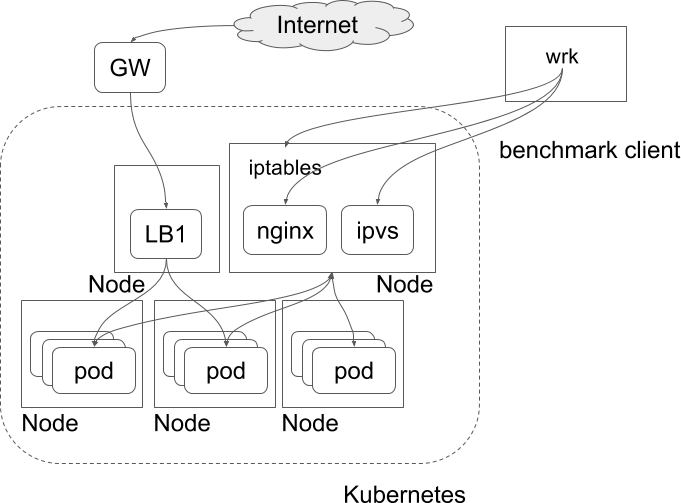
\includegraphics[width=0.8\columnwidth]{Figs/benchmark-schem}
  \vspace{1cm}
  \caption{Logical configuration.}
  \label{fig:benchmark-schem}
\end{subfigure}
  \vspace{1cm}

\begin{subfigure}[t]{\columnwidth}
  \centering
  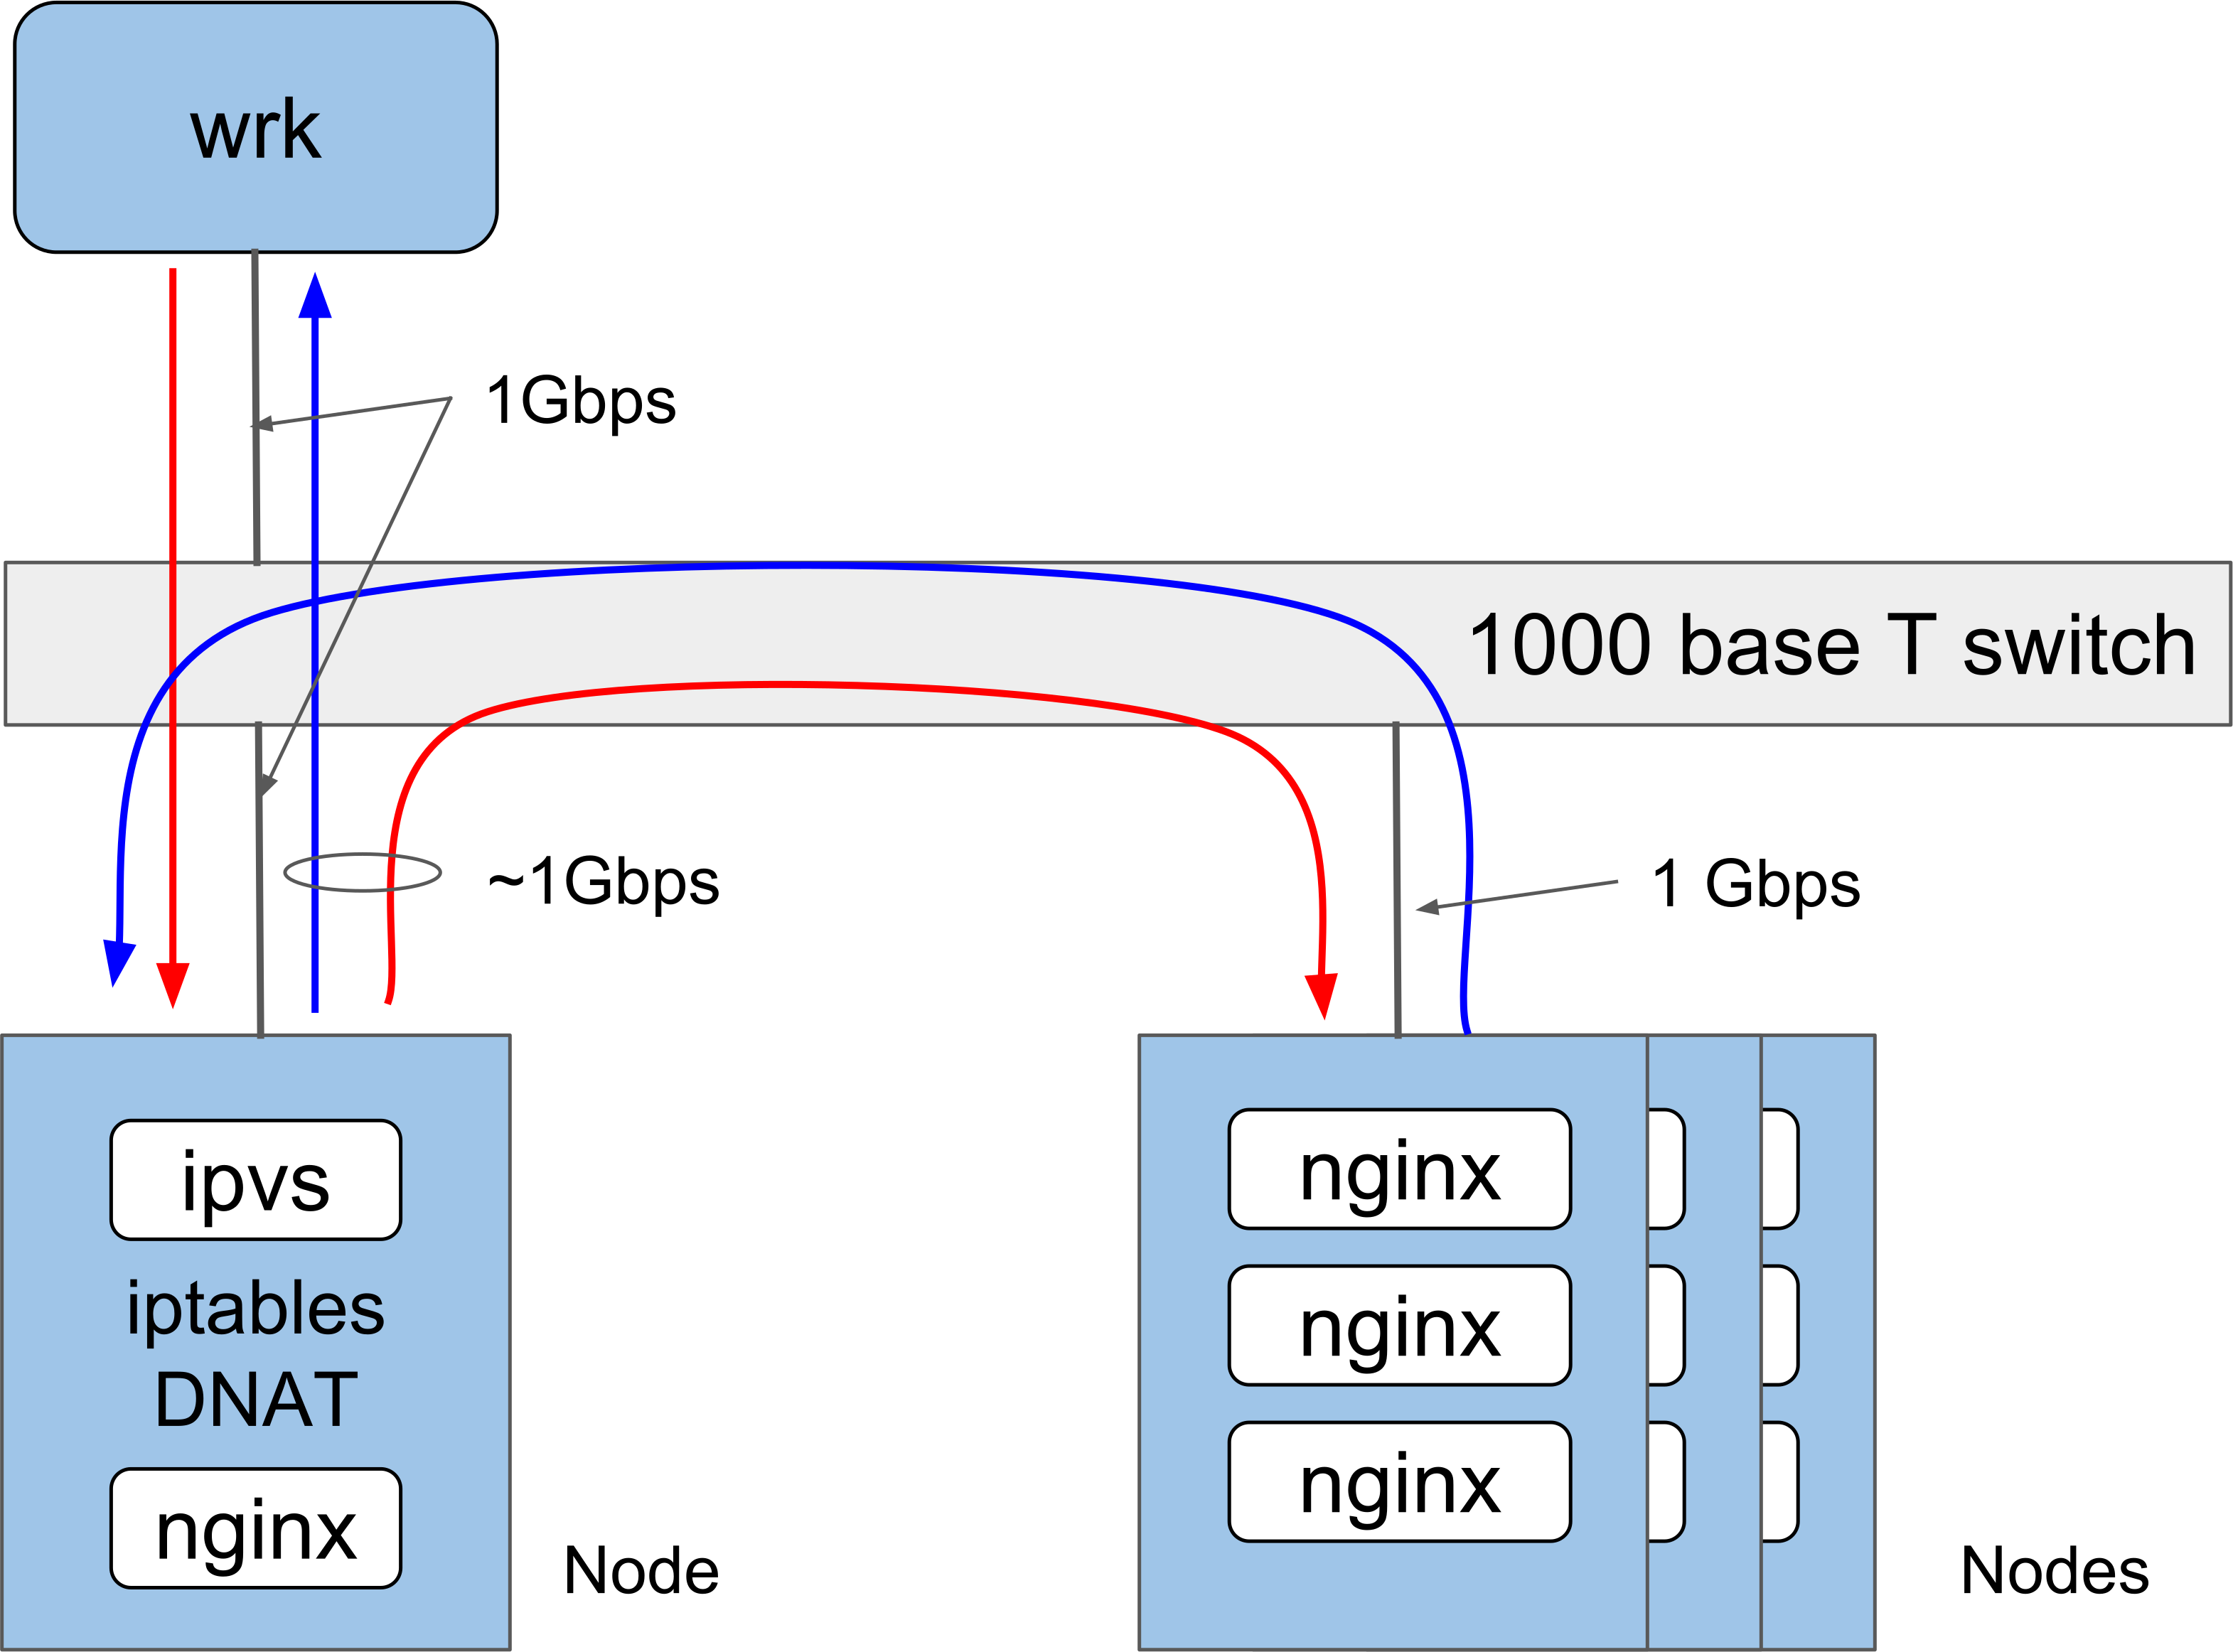
\includegraphics[width=0.8\columnwidth]{Figs/bench_1g}
  \vspace{1cm}
  \caption{Physical configuration.}
  \label{fig:bench_1g}
\end{subfigure}
  \caption{Benchmark setup. }
  \label{fig:benchmark-setup}
\end{figure}

Table~\ref{tab:bench_example} shows an example of the command-line for wrk and the corresponding output.
The command-line in Table~\ref{tab:bench_example} will generate 40 wrk program threads and allow those threads to send out a total of 800 concurrent HTTP requests over the period of 30 seconds.
The output example shows the information including per thread statistics, error counts, Request/sec and Transfer/sec.

\begin{table}[h]
  \centering
  \begin{tabular}{l}
    \hline
    \begin{minipage}{13cm}
      \begin{verbatim}

[Command line] 
 wrk -c800 -t40 -d30s http://172.16.72.2:8888/ 
-c: concurrency, -t: # of thread, -d: duration 

[Output example] 
 Running 30s test @ http://10.254.0.10:81/ 
  40 threads and 800 connections 
  Thread Stats   Avg      Stdev     Max   +/- Stdev 
    Latency    15.82ms   41.45ms   1.90s    91.90\% 
    Req/Sec     4.14k   342.26     6.45k    69.24\% 
  4958000 requests in 30.10s, 1.14GB read 
  Socket errors: connect 0, read 0, write 0, timeout 1 
Requests/sec: 164717.63 
Transfer/sec:     38.86MB 
      \end{verbatim}
    \end{minipage}
   \\ \hline
  \end{tabular}
  \caption{}
  \label{tab:bench_example}
\end{table}

Table~\ref{tab:hw_sw_spec} shows hardware and software configuration used in the experiments.
%Physical servers with the same specification are used for nodes(nginx, load balancer) and benchmark client.
All of the nginx web server pods are configured to return the IP address of the {\em pod}, in order to make them return a small HTTP content. This makes a relatively severe condition for load balancers. 
The size of the character string making up an IP address is limited to 15 bytes.
If the author had chosen the HTTP response size so that most of the IP packet resulted in maximum transmission unit(MTU), the performance would have been dominantly limited by the Ethernet bandwidth.
However, since small HTTP responses are used, the auhtor could purely measure the load balancer performance.

\begin{table}[]
  \centering
  \begin{tabular}{ll}
    \hline 
    \multicolumn{2}{l}{[Hardware Specification]}   \\
    & CPU: Xeon E5-2450 2.10GHz (with 8 core, Hyper Threading) \\
    & Memory: 32GB \\
    & NIC: Broadcom BCM5720 Giga bit \\
    & (Node x 6, LB x 1, Client x 1) \\
    & \\
    \multicolumn{2}{l}{[Node Software]}  \\
    & OS: Debian 8.7, linux-3.16.0-4-amd64 \\
    & Kubernetes v1.10.6 \\
    & flannel v0.7.0 \\
    & etcd version: 3.0.15 \\
    & \\
    \multicolumn{2}{l}{[Container Software]}   \\
    & Keepalived: v1.3.2 (12/03,2016) \\
    & nginx : 1.11.1(load balancer), 1.13.0(web server) \\
    \hline
  \end{tabular}
  \caption{}
  \label{tab:hw_sw_spec}
\end{table}

For this experiment a total of eight servers are used; six servers for nodes, one for the load balancer and one for the benchmark client, with all having the same hardware specifications.
The software versions used for Kubernetes, web server and load balancer {\em pods} are also summarized in the Table~\ref{tab:hw_sw_spec}.
The hardware we used had eight physical CPU cores and a 1Gbps NIC with 4 rx-queues.

\subsection{Result 1: Effect of multicore proccessing}

\begin{figure}
  \centering
  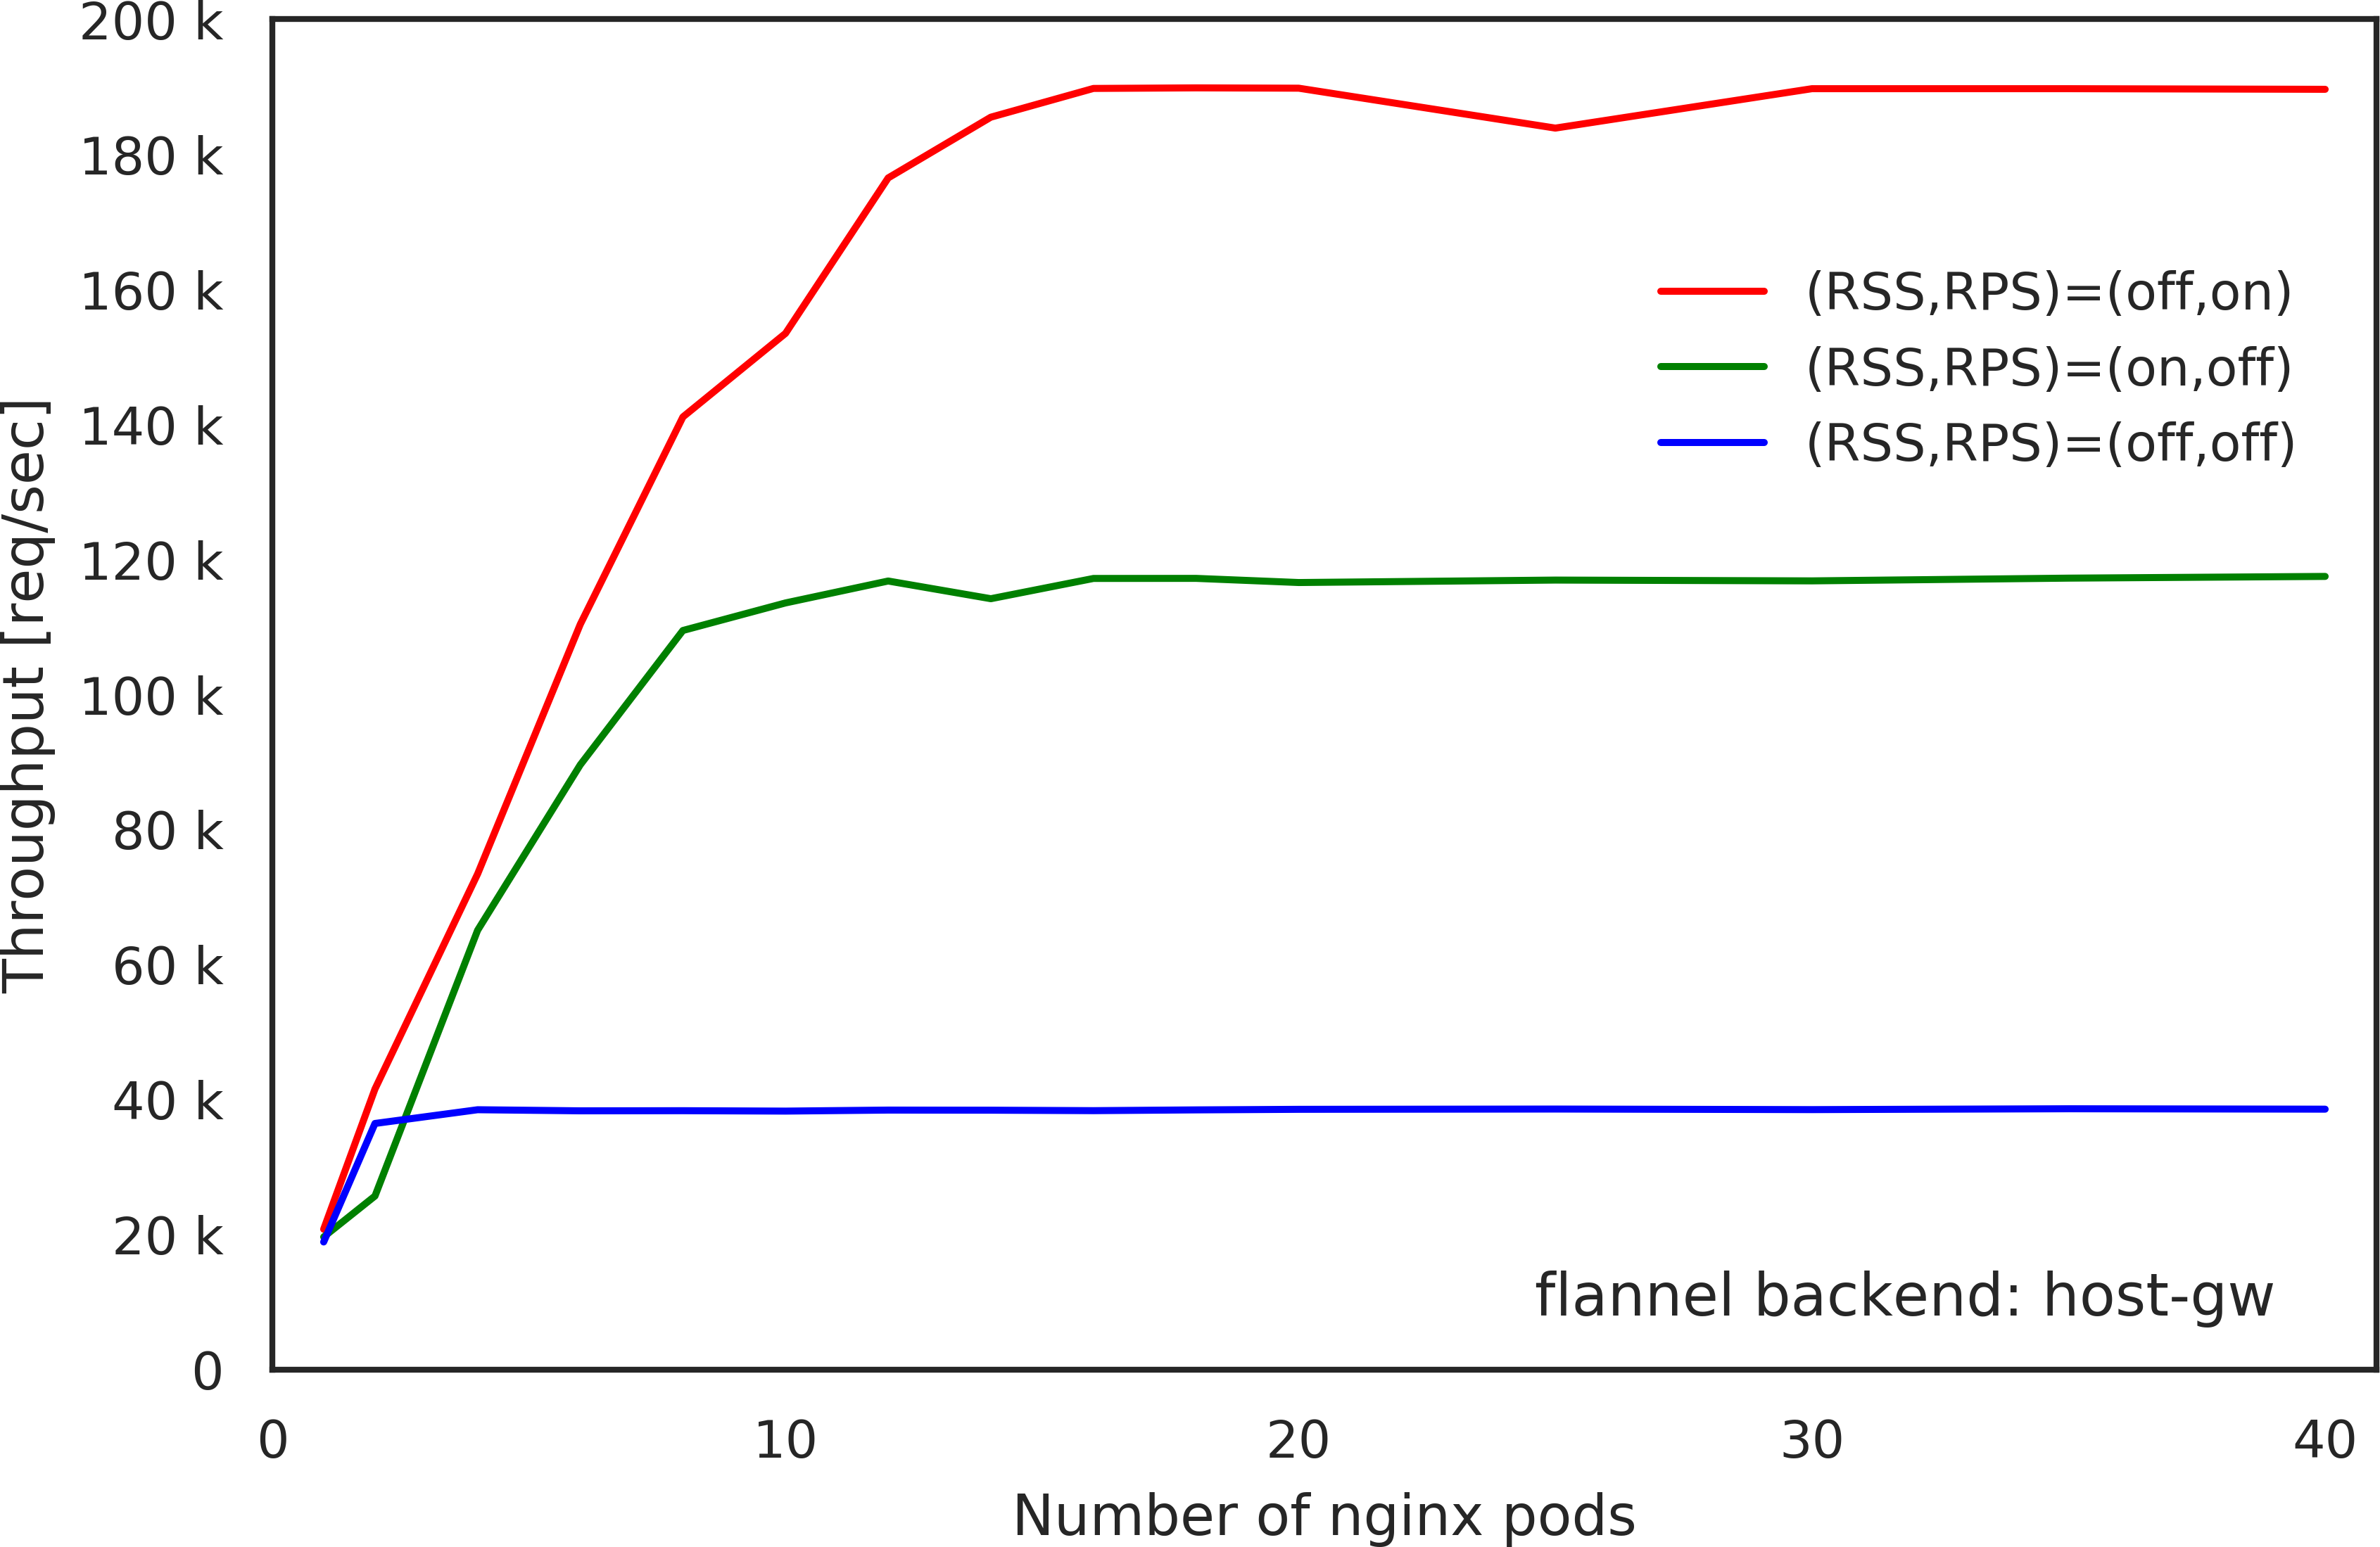
\includegraphics[width=0.8\columnwidth]{Figs/ipvs_mcore_proccessing}
  \caption{Effect of multicore proccessing on ipvs throughput.}
  \label{fig:ipvs_mcore_proccessing}
\end{figure}

Figure~\ref{fig:ipvs_mcore_proccessing} shows the effect of multicore proccessing.
The following three RSS and RPS settings were compared: 
\begin{center}
  \centering
  \begin{minipage}{0.8\columnwidth}
\begin{verbatim}
(RSS, RPS) = (off, off)
           = (on , off)
           = (off, on )
\end{verbatim}
  \end{minipage}
\end{center}
The host-gw mode of flannel backends is used as the overlay network.

We can see a general trend in which the throughput linearly increases as the number of nginx {\em pod}s increases and then it eventually saturates.
The saturated throughput levels indicate the maximum performance level of the ipvs load balancer.
The maximum performance levels depend on the (RSS, RPS) settings.
From the results in this figure, it can be seen that if we turn off distributed packet processing,
{\it i.e.}, when \enquote{(RSS, RPS) = (off, off)}, performance degrades significantly.
In this case, the performance bottleneck is primarily due to packet processing in a single core.

If we compare the results for the cases when \enquote{(RSS, RPS) = (on, off)} and \enquote{(RSS, RPS) = (off, on)},
the latter is better than the former.
This is understandable, since in the case of \enquote{(RSS, RPS) = (off, on)}, eight physical cores can be used whereas 
in the case of \enquote{(RSS, RPS) = (on, off)} only four cores can be used, on the hardware used in our experiment.
The performance bottleneck of the case when \enquote{(RSS, RPS) = (on, off)} is considered 
to be due to the fact that the packet processing is only done on four CPU cores.
It can be said that \enquote{(RSS, RPS) = (off, on)} is the best setting in our experimental conditions, and the author used this setting throughout this thesis unless explicitly stated otherwise.

\subsection{Result 2: Effect of overlay network}

\begin{figure}[h]
  \centering
  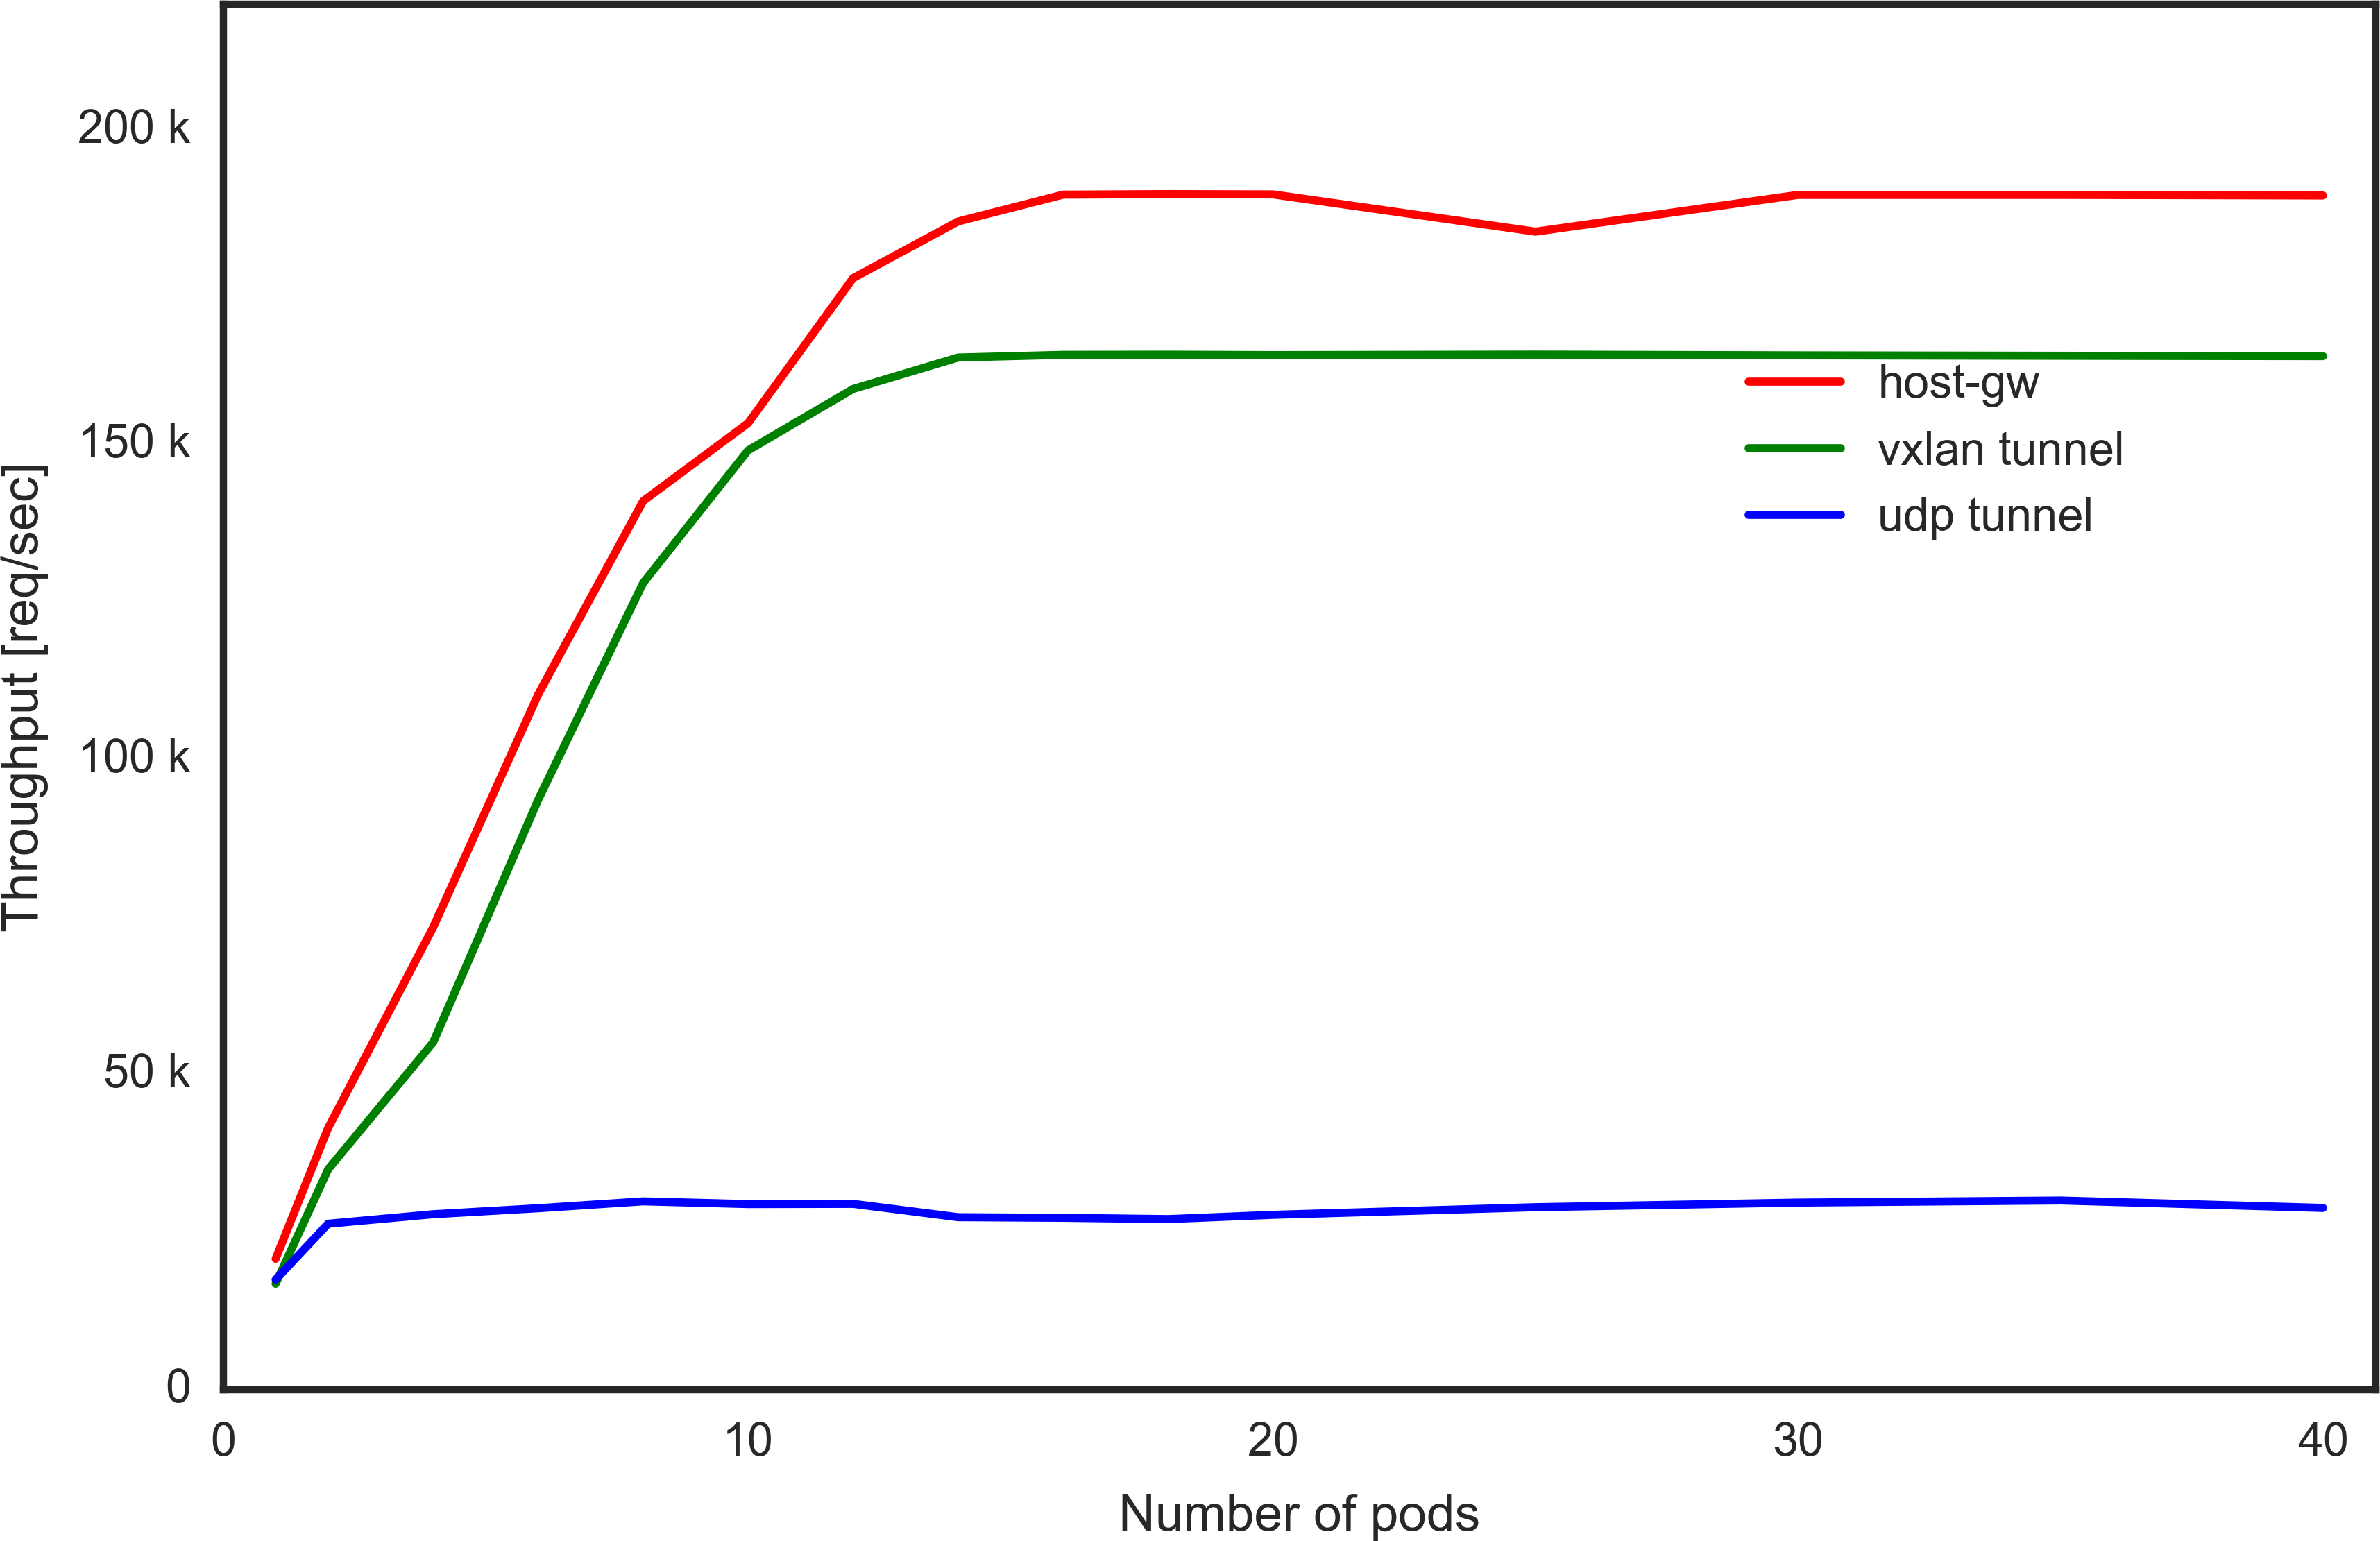
\includegraphics[width=0.8\columnwidth]{Figs/ipvs_flannel_mode}
  \caption{Effect of flannel backend modes on ipvs throughput.}
  \label{fig:ipvs_flannel_mode}
\end{figure}

Figure~\ref{fig:ipvs_flannel_mode} shows the effect of flannel backend modes on ipvs throughput.
As for the overlay network, the author measured the performance levels for three flannel backend modes, host-gw, vxlan and udp .
Except for the udp cases, we can see the trend in which the throughput linearly increases 
as the number of nginx {\em pod} increases and then it eventually saturates.
The saturated performance levels indicates the maximum performance of the ipvs load balancer.
If we compare the performance levels among the flannel backend modes types, 
the host-gw mode where no encapsulation is conducted shows the highest performance level,
followed by the vxlan mode where the Linux kernel encapsulate the Ethernet frame.
The udp mode where flanneld itself encapsulate the IP packet shows significantly lower performances levels.

\subsection{Result 3: Comparison of different load balancer}

\begin{figure}[h]
  \centering
  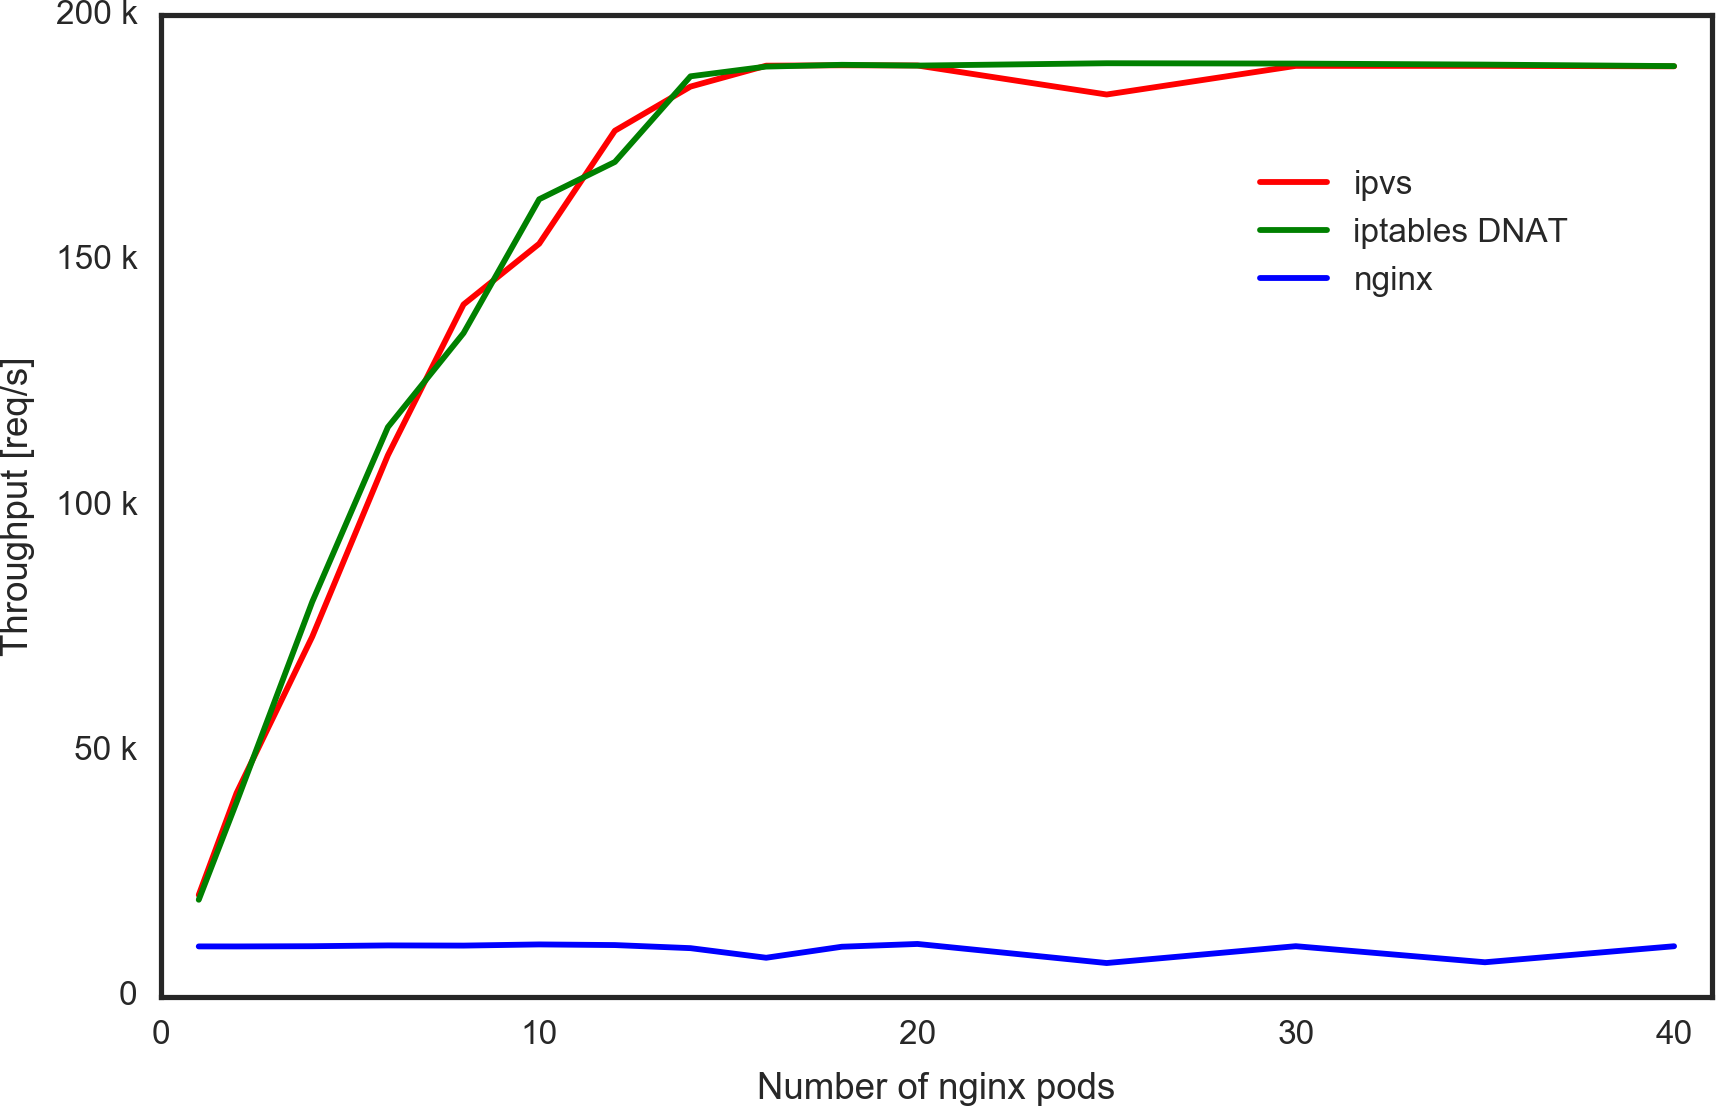
\includegraphics[width=0.8\columnwidth]{Figs/ipvs-iptables-nginx}
  \caption{Throughput comparison between ipvs, iptables DNAT and nginx. The host-gw of the flannel backend modes and a kernel setting of \enquote{(RSS, RPS) = (off on)} for multicore packet proccessing is used. }
  \label{fig:ipvs-iptables-nginx}
\end{figure}

\begin{figure}[h]
  \centering
  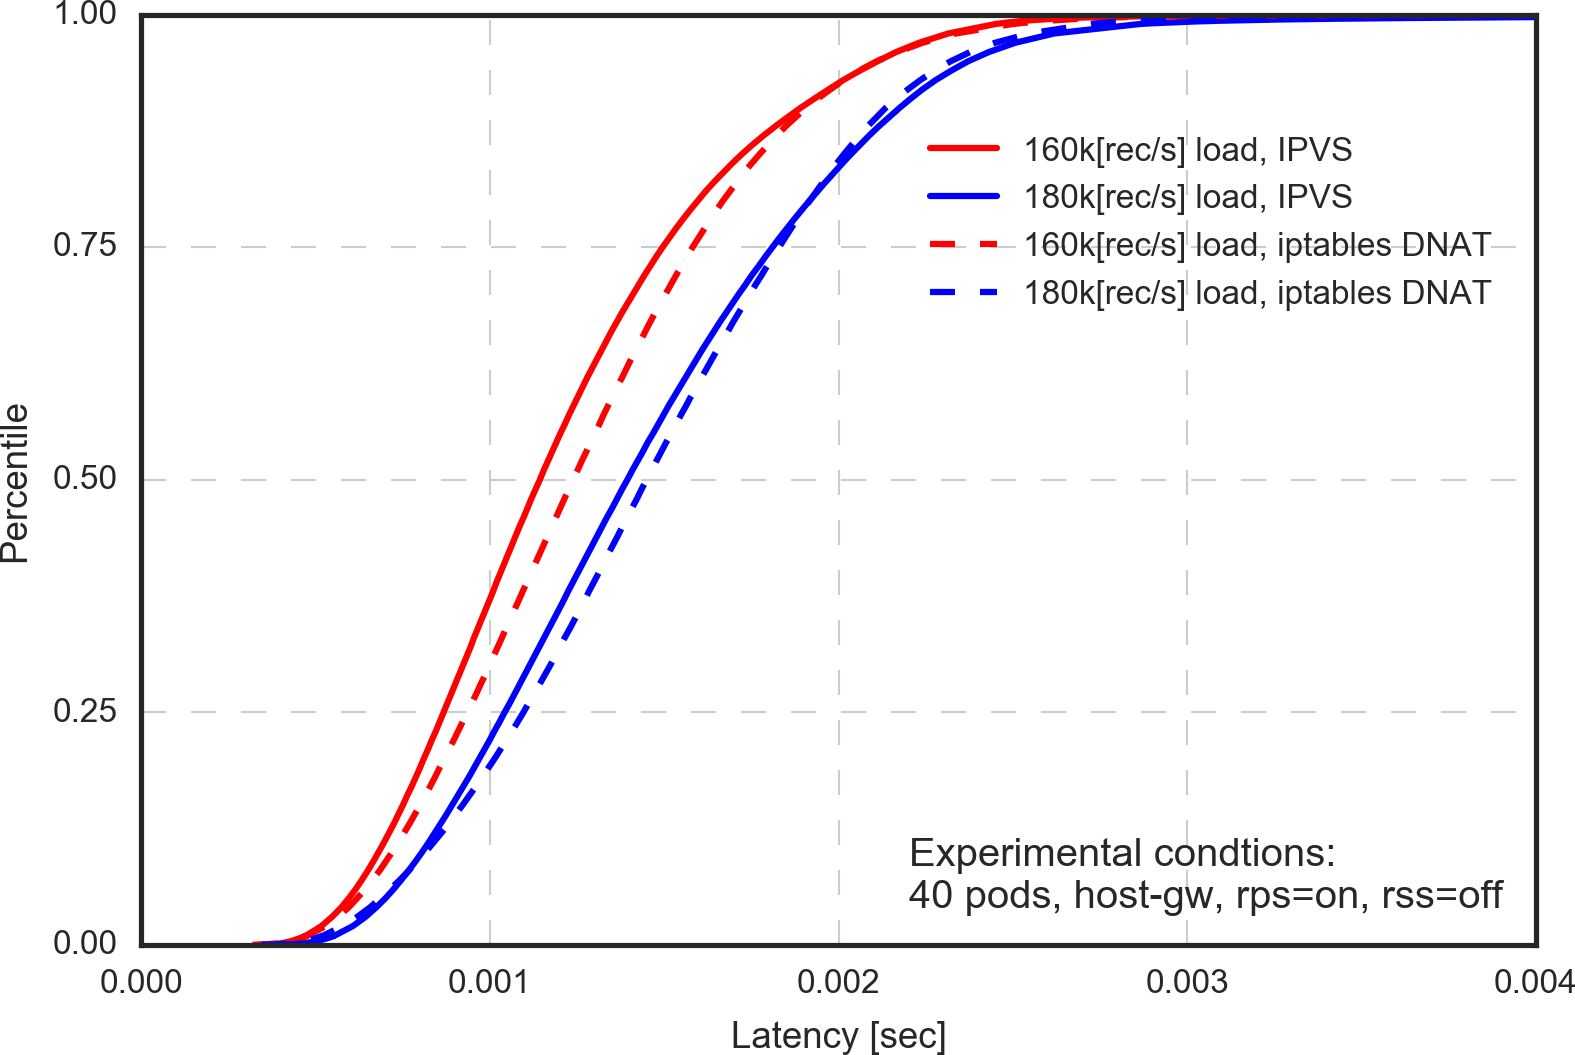
\includegraphics[width=0.8\columnwidth]{Figs/latency_cdf_rps_40pods}
  \caption{Latency cumulative distribution function.}
  \label{fig:latency_cdf_rps_40pods}
\end{figure}

Figure~\ref{fig:ipvs-iptables-nginx} compares the performance measurement results among the ipvs, iptables DNAT, and Nginx load balancers.
The proposed ipvs load balancer exhibits almost equivalent performance as the iptables DNAT based load balancer. 
The Nginx based load balancer shows no performance improvement even though the number of the Nginx web server {\em pods} is increased.
It is understandable because the performance of the single nginx as a load balancer is expected to be similar to the performance as a web server.

Figure~\ref{fig:latency_cdf_rps_40pods} compares Cumulative Distribution Function(CDF) of the load balancer latency at the two constant loads, 160K[req/sec] and 180K[req/sec].
We can see that the latencies are a little bit smaller for ipvs.
For example, the median value at 160K[req/sec] load for ipvs and iptables DNAT are, 1.1 msec and 1.2 msec, respectively.
This may not be considered a siginificant difference, however we can at least say that our proposed load balancer are as good as iptables DNAT.

\subsection{Analysis of the performance limitation}

\begin{lstlisting}[
    backgroundcolor = \color{mygray},
    basicstyle=\footnotesize,
    breaklines=true,
    numbers=left,
    %    postbreak=\mbox{\textcolor{red}{$\hookrightarrow$}\space},
    caption={An example of the tcpdump output},
    captionpos=b,
    label={list:tcpdump}
  ]
  curl -s  http://172.16.72.2:8888/1000
  tcpdmup(response):

  03:09:27.968942 IP 172.16.72.2.8888 > 192.168.0.112.60142:
  Flags [S.], seq 2317920646, ack 648140715, win 28960, options [mss 1460,sackOK,TS val 2274012282 ecr 2324675546,nop,wscale 8], length 0
  03:09:27.969685 IP 172.16.72.2.8888 > 192.168.0.112.60142:
  Flags [.], ack 85, win 114, options [nop,nop,TS val 2274012282 ecr 2324675546], length 0
  03:09:27.969945 IP 172.16.72.2.8888 > 192.168.0.112.60142:
  Flags [P.], seq 1:255, ack 85, win 114, options [nop,nop,TS val 2274012282 ecr 2324675546], length 254
  03:09:27.969948 IP 172.16.72.2.8888 > 192.168.0.112.60142:
  Flags [P.], seq 255:1255, ack 85, win 114, options [nop,nop,TS val 2274012282 ecr 2324675546], length 1000
  03:09:27.970846 IP 172.16.72.2.8888 > 192.168.0.112.60142:
  Flags [F.], seq 1255, ack 86, win 114, options [nop,nop,TS val 2274012282 ecr 2324675547], length 0
\end{lstlisting}

\begin{table}[h]
\centering
  \begin{tabular}{|l|r|r|r|r|}
    \hline
%    \multicolumn{5}{|l|}{Data size in 100 HTTP requests.} \\ \hline
    Type of Packet & \multicolumn{1}{l|}{Payload {[}byte{]}} & \multicolumn{1}{l|}{Header {[}byte{]}} & \multicolumn{1}{l|}{Count} & \multicolumn{1}{l|}{Total {[}byte{]}} \\ \hline
    SYN & 0 & 98 & 1 & 98 \\ \hline
    ACK & 0 & 90 & 102 & 9,180 \\ \hline
    Push(GET) & 44 & 90 & 100 & 13,400 \\ \hline
    FIN+ACK & 0 & 90 & 1 & 90 \\ \hline
    \multicolumn{3}{|l|}{Total} & \multicolumn{2}{r|}{22,768} \\ \hline
  \end{tabular}
  \caption{Request data size for 100 HTTP requests in wrk measurement.}
  \label{tab:request_data_size}
%% \end{table}

  \vspace{1cm}
  
%% \begin{table}[h]
\centering
  \begin{tabular}{|l|r|r|r|r|}
    \hline
%    \multicolumn{5}{|l|}{Response Data size for 100 HTTP requests in wrk measurement.} \\ \hline
    Type of Packet & \multicolumn{1}{l|}{Payload {[}byte{]}} & \multicolumn{1}{l|}{Header {[}byte{]}} & \multicolumn{1}{l|}{Count} & \multicolumn{1}{l|}{Total {[}byte{]}} \\ \hline
    SYN+ACK & 0 & 98 & 1 & 98 \\ \hline
    ACK & 0 & 90 & 2 & 180 \\ \hline
    Push(GET) & 254 & 90 & 100 & 34,400 \\ \hline
    Push(DATA) & data & 90 & 100 & 100x(data+90) \\ \hline
    FIN+ACK & 0 & 90 & 1 & 90 \\ \hline
    \multicolumn{3}{|l|}{Total} & \multicolumn{2}{r|}{100x(data+90)+34,768} \\ \hline
  \end{tabular}
  \caption{Response data size for 100 HTTP requests in wrk measurement.}
  \label{tab:response_data_size}
\end{table}

\begin{table}[h]
\begin{center}
  \begin{tabular}{|l|r|r|}
    \hline
    Type of field & \multicolumn{1}{l|}{SYN} & \multicolumn{1}{l|}{\begin{tabular}[c]{@{}l@{}}ACK, SYN+ACK,\\ FIN+ACK, PUSH\end{tabular}} \\ \hline
    preamble & 8 & 8 \\ \hline
    ether header & 14 & 14 \\ \hline
    ip header & 20 & 20 \\ \hline
    tcp header & 20 + 20(tcp options) & 20 + 12(tcp options) \\ \hline
    fcs & 4 & 4 \\ \hline
    inter frame gap & 12 & 12 \\ \hline
    Total [byte] & 98 & 90 \\ \hline
  \end{tabular}
  \caption{Header sizes of TCP/IP packet in Ethernet frame.}
  \label{tab:header_size}
\end{center}
\end{table}

\begin{figure}[h]
  \centering
  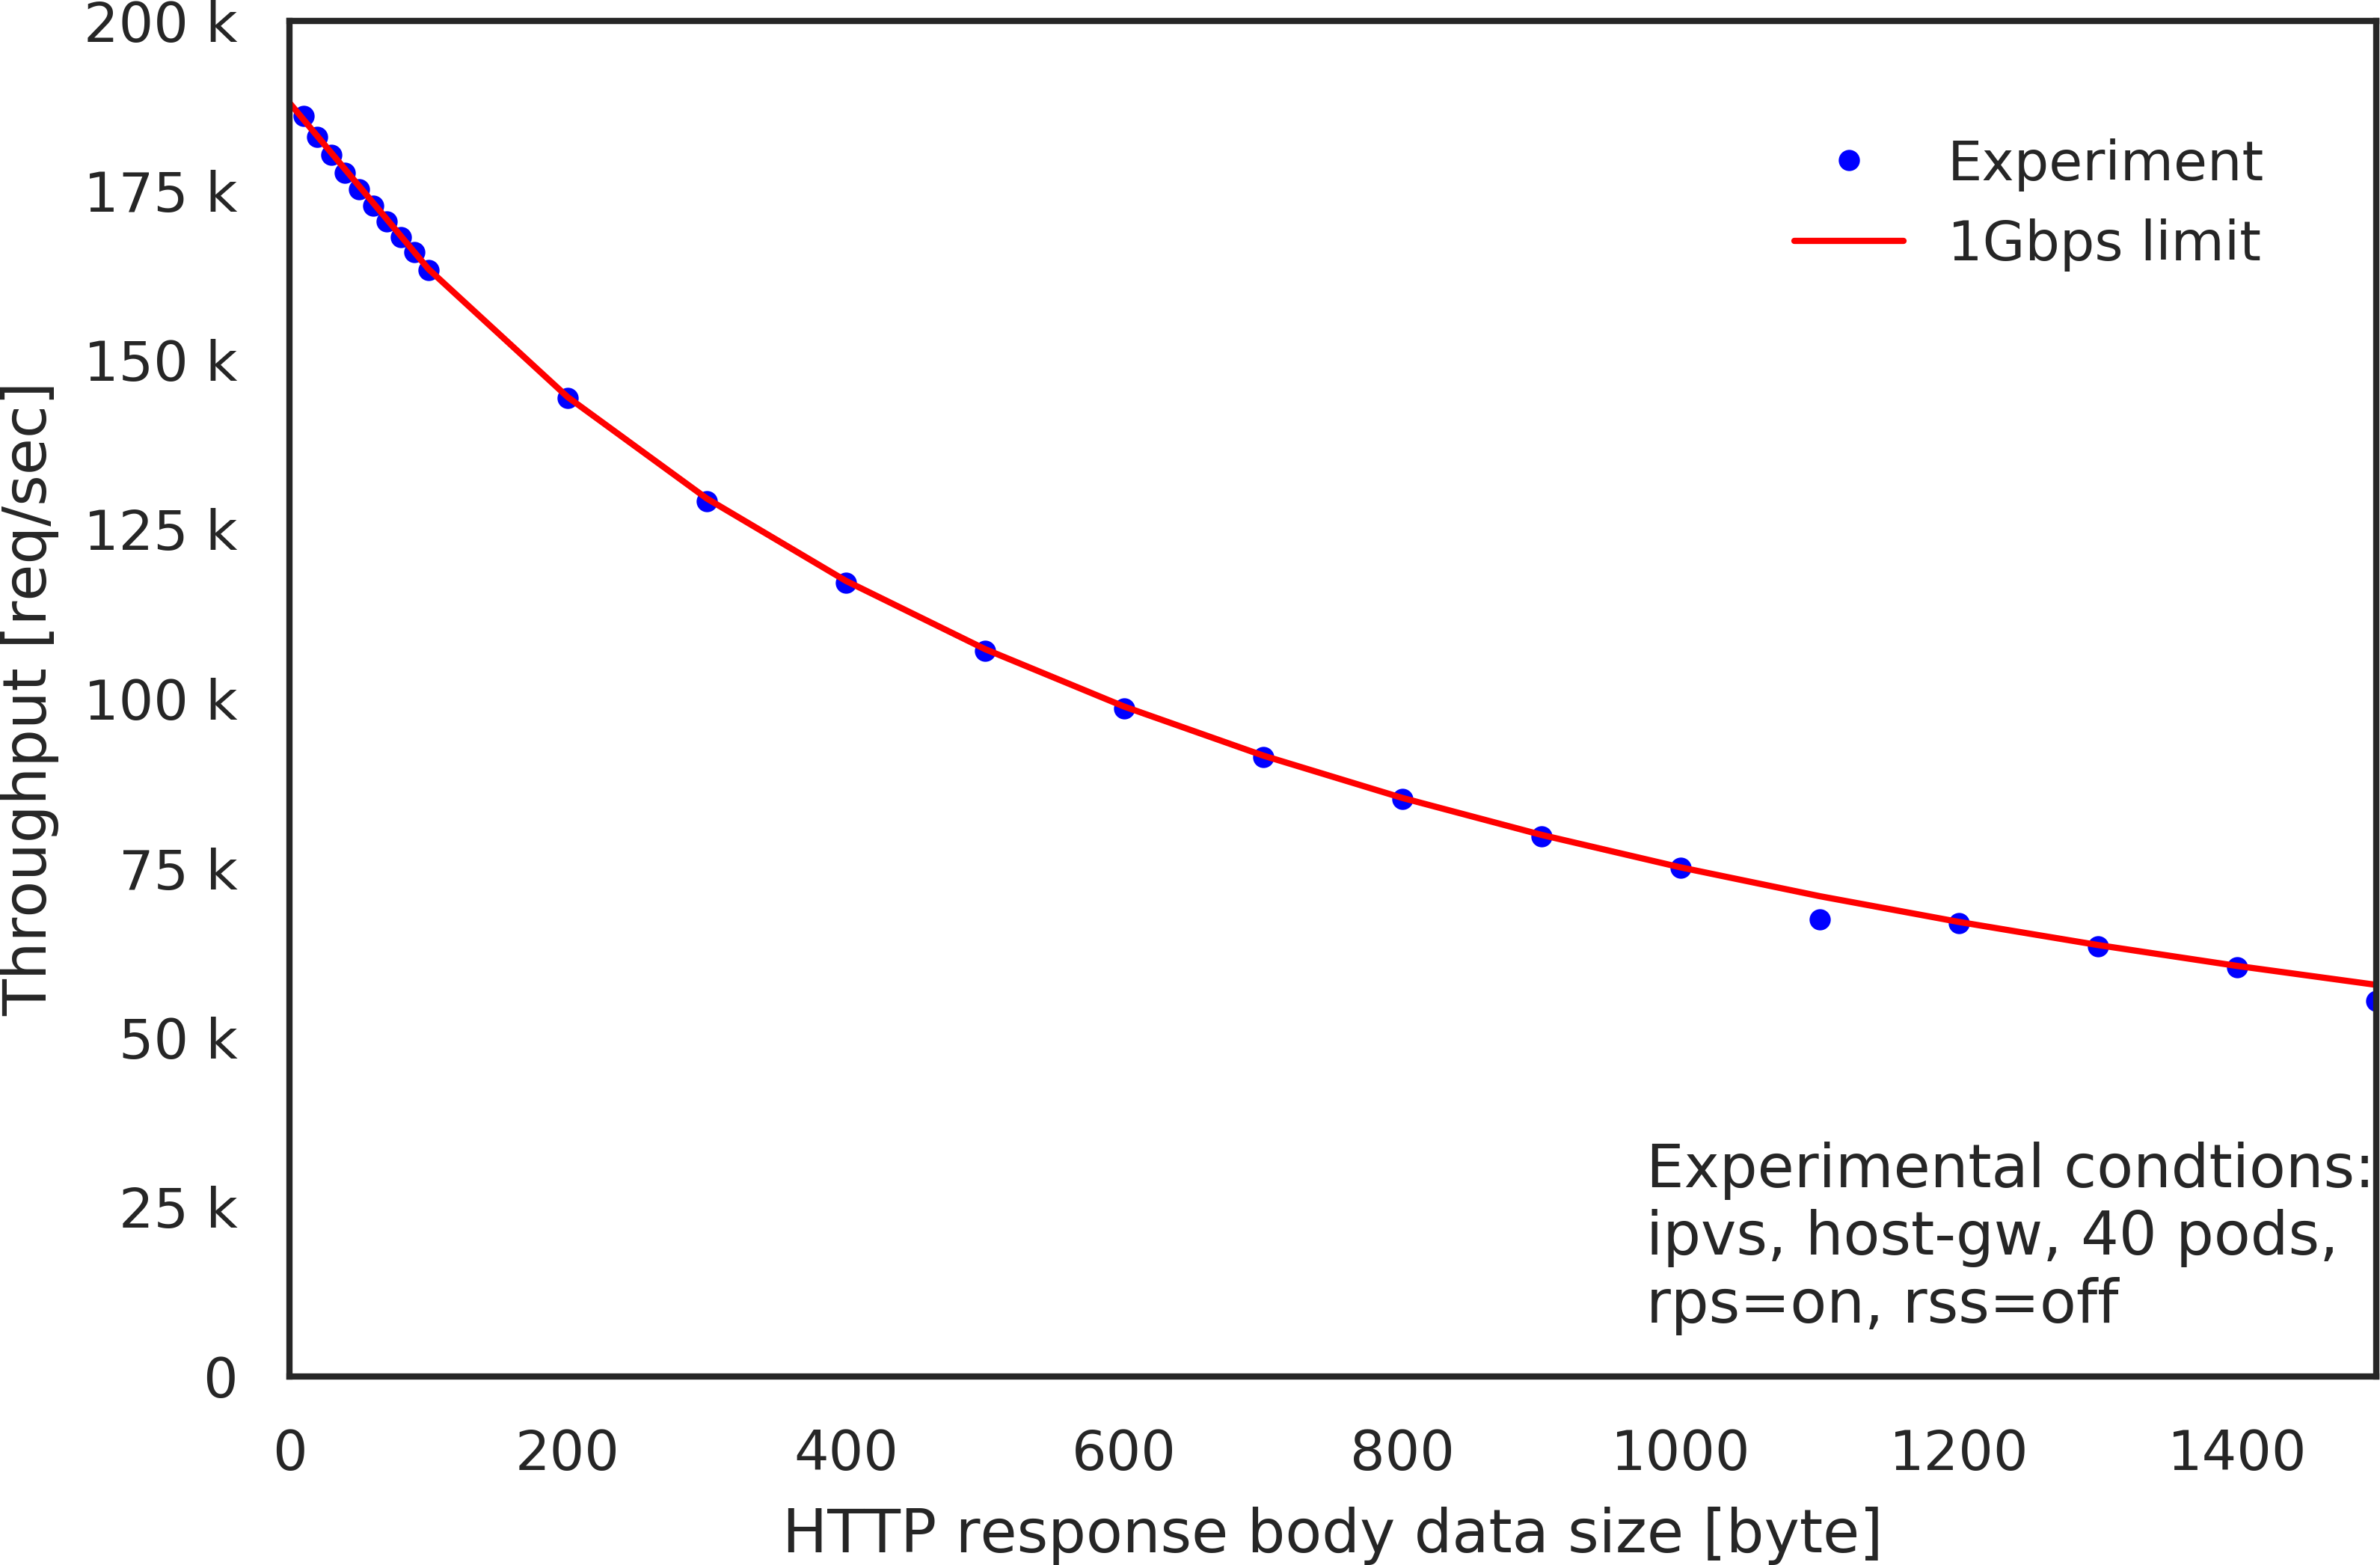
\includegraphics[width=0.8\columnwidth]{Figs/tp_limit_1gbps}
  \caption{Performance limitation due to 1Gbps bandwidth}
  \label{fig:performance_limitation}
\end{figure}

The maximum throghput in this series of experiment is roughly, 190k[req/sec] for both ipvs an the iptables DNAT.
At first, it was not clear what caused this limitation.
The author analyzed the kind of packets that flows during the experiment using tcpdump\cite{jacobson1989tcpdump} as follows;
1) A wrk worker opens multiple connections and sends out http request to the web servers. The number of connections is determined by the command-line option, eg. 800/40 = 20 connection in the case of command-line in Table~\ref{tab:bench_example}. The worker sends out 100 requests to the web server within each connection, and closes it either if all of the responses are recieved or time out occurs.
2) As in seen in Listing~\ref{list:tcpdump}, tcp options were mss(4 byte), sack(2 byte), ts(10 byte), nop(1 byte) and wscale(3 byte), for SYN packets. For other packets, tcp options were, nop(1 byte), nop(1 byte) and ts(10 byte).
3) The author classified the types of packes and counted the number of each type in a single connection, which is 100 http requests. Table~\ref{tab:response_data_size},\ref{tab:response_data_size},\ref{tab:header_size} summarize the data size of 100 request, including TCP headr, IP header, Ether header and overheads. 
From this analysis, it was found that per each HTTP request and response,
request data with the size of 227.68[byte] and response data with the data(http content)+437.68[byte] were being sent.   

Since the node for load balancer recives and transmits both request and response packets using single network interface, each 1Gbps half duplex of full duplex must accomodate request and response data size.
Therefore the theoretical maximum throughput can be expressed as; \\
throughput[req/sec] = band width[byte/sec]/(request + response) \\
= 1e9/8/(data+665.36)

Figure~\ref{fig:performance_limitation} shows plot of theoretical maximum throughput 1Gbps ethernet together with actual benchmark results.
Since experimnetal results agrees well with theory, the author concludes that when \enquote{RPS = on}, ipvs performance limitation is due to the 1Gbps bandwidth.


\section{On-premise experiment with 10Gbps Load balancer}

\begin{figure}[t]
  \centering
  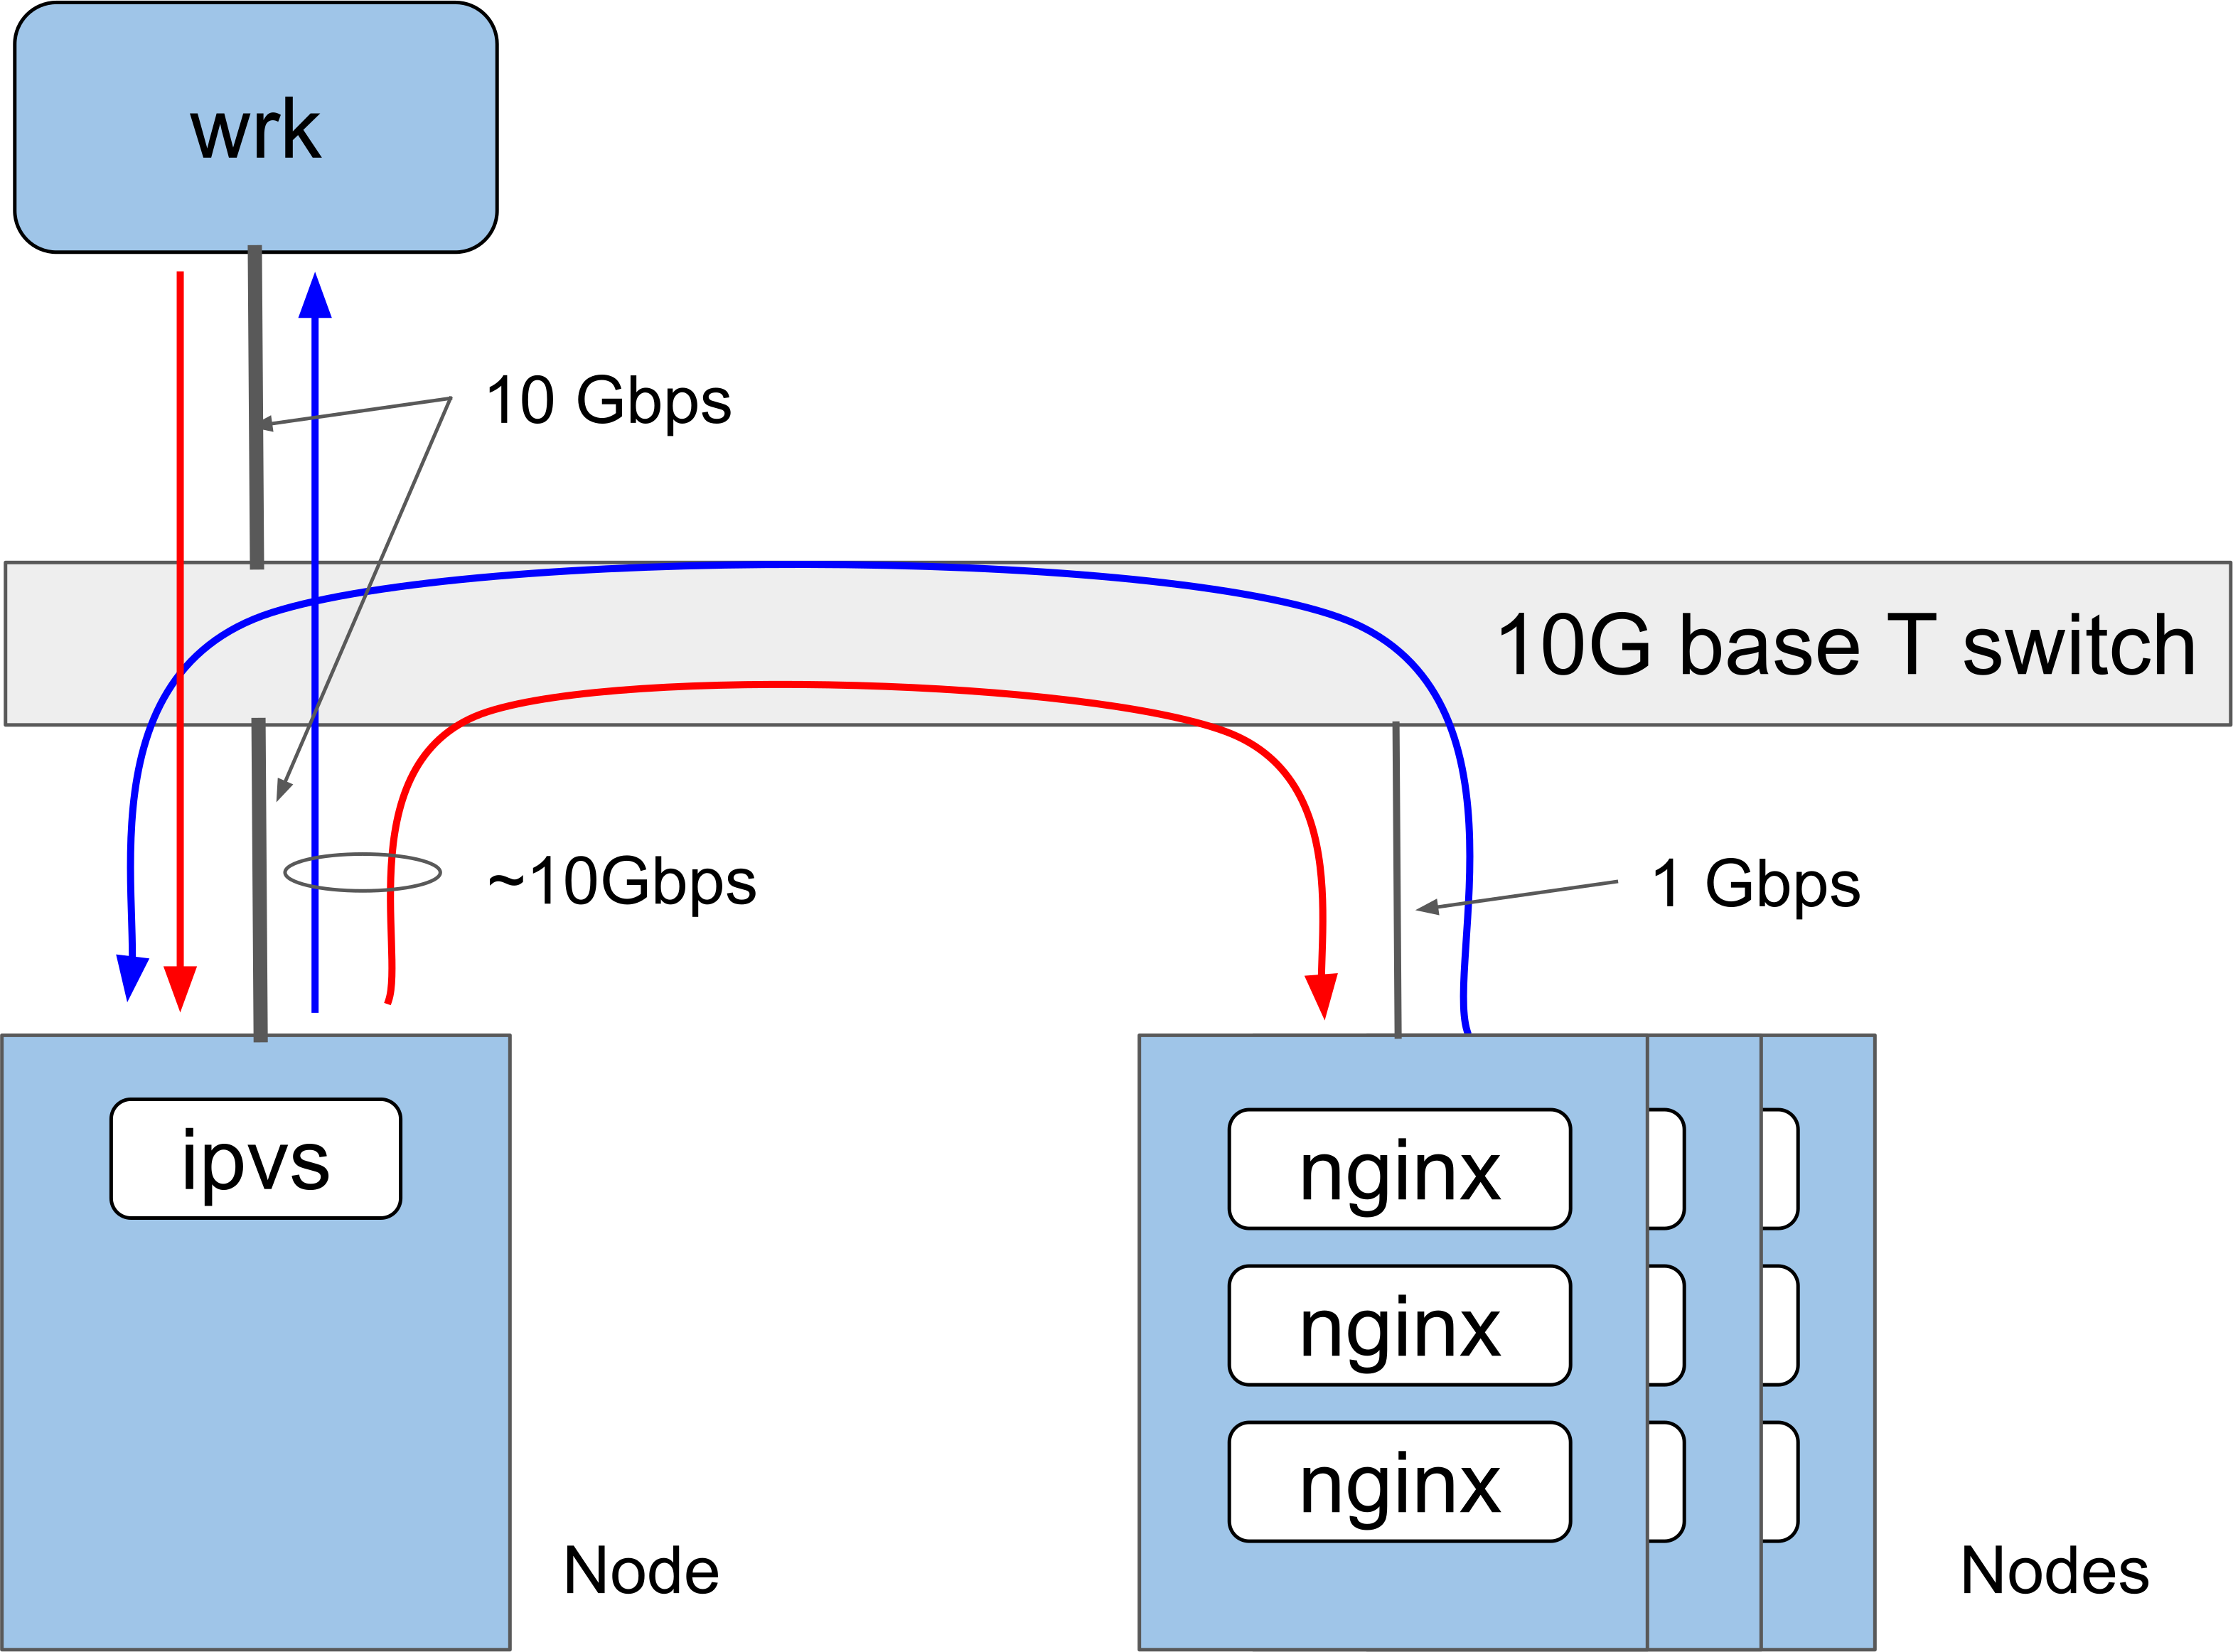
\includegraphics[width=0.8\columnwidth]{Figs/bench_10g}
  \caption{Physical configuration for 10Gbps measurement.}
  \label{fig:bench_10g}
\end{figure}

\begin{figure}[t]
  \centering
  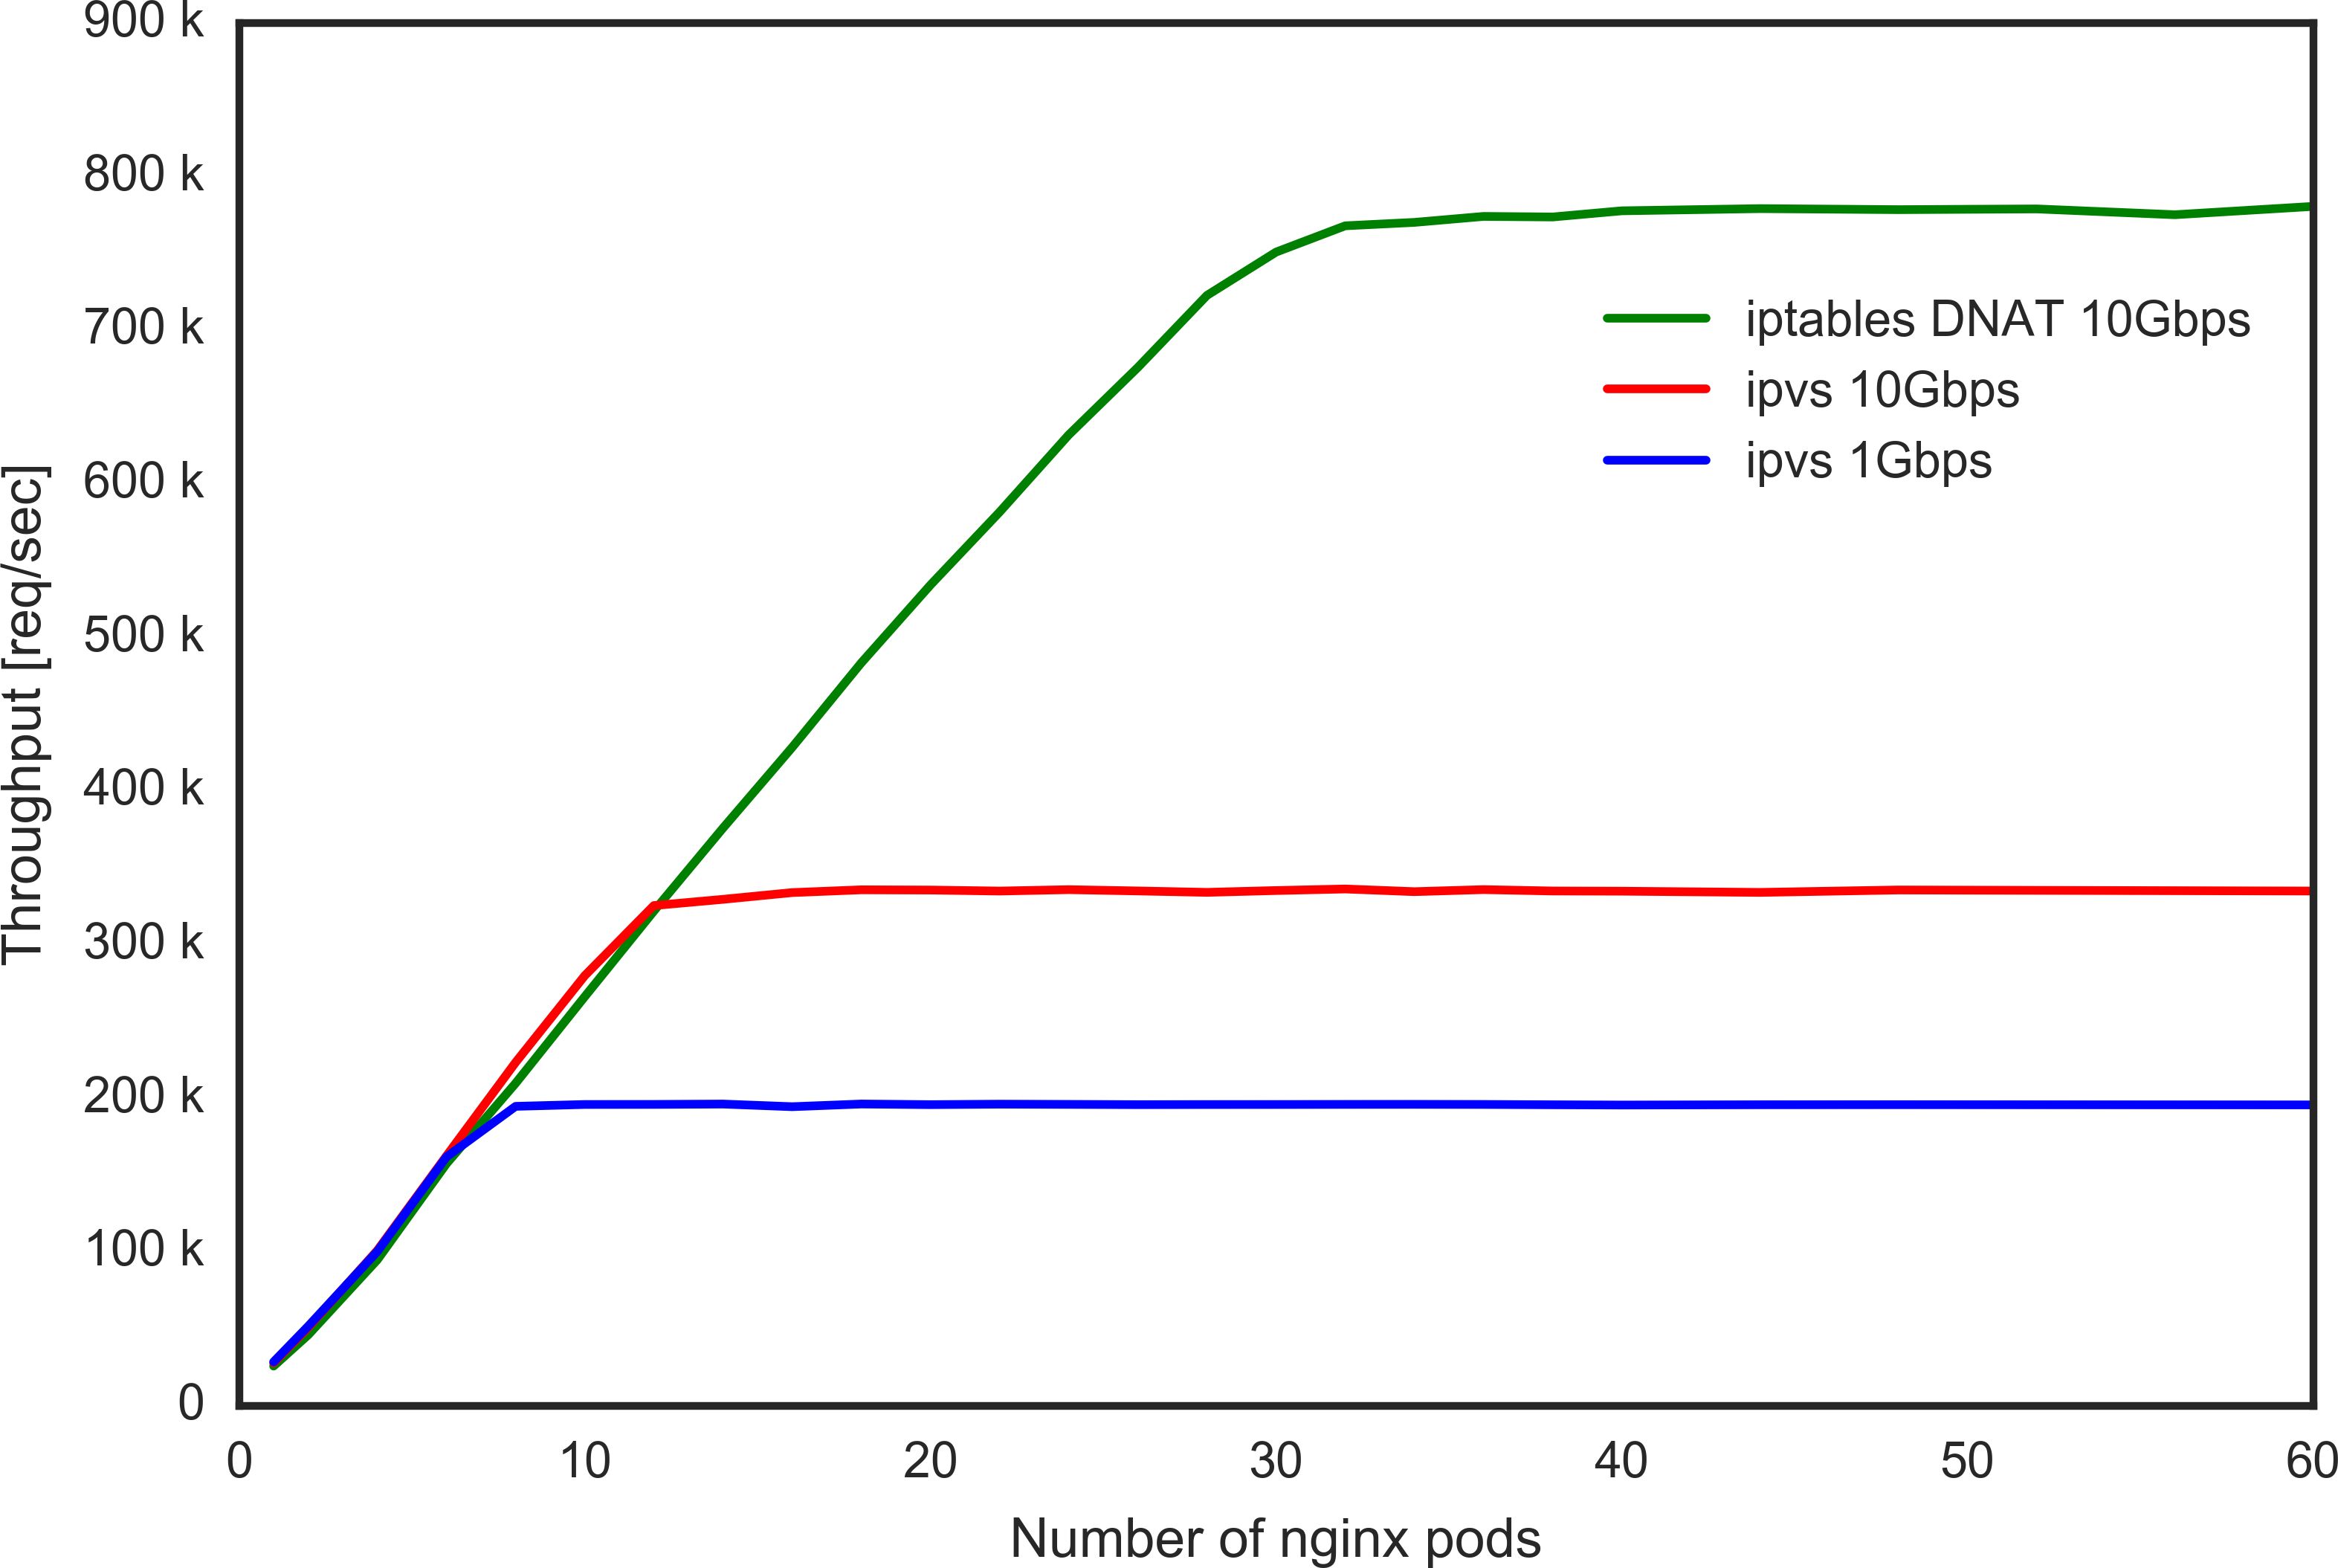
\includegraphics[width=0.8\columnwidth]{Figs/ipvs_iptables_dnat_10g}
  \caption{comparison between ipvs and iptables @10Gbps.}
  \label{fig:ipvs_iptables_dnat_10g}
\end{figure}

\section{L3DSR}

\begin{figure}[t]
  \centering
  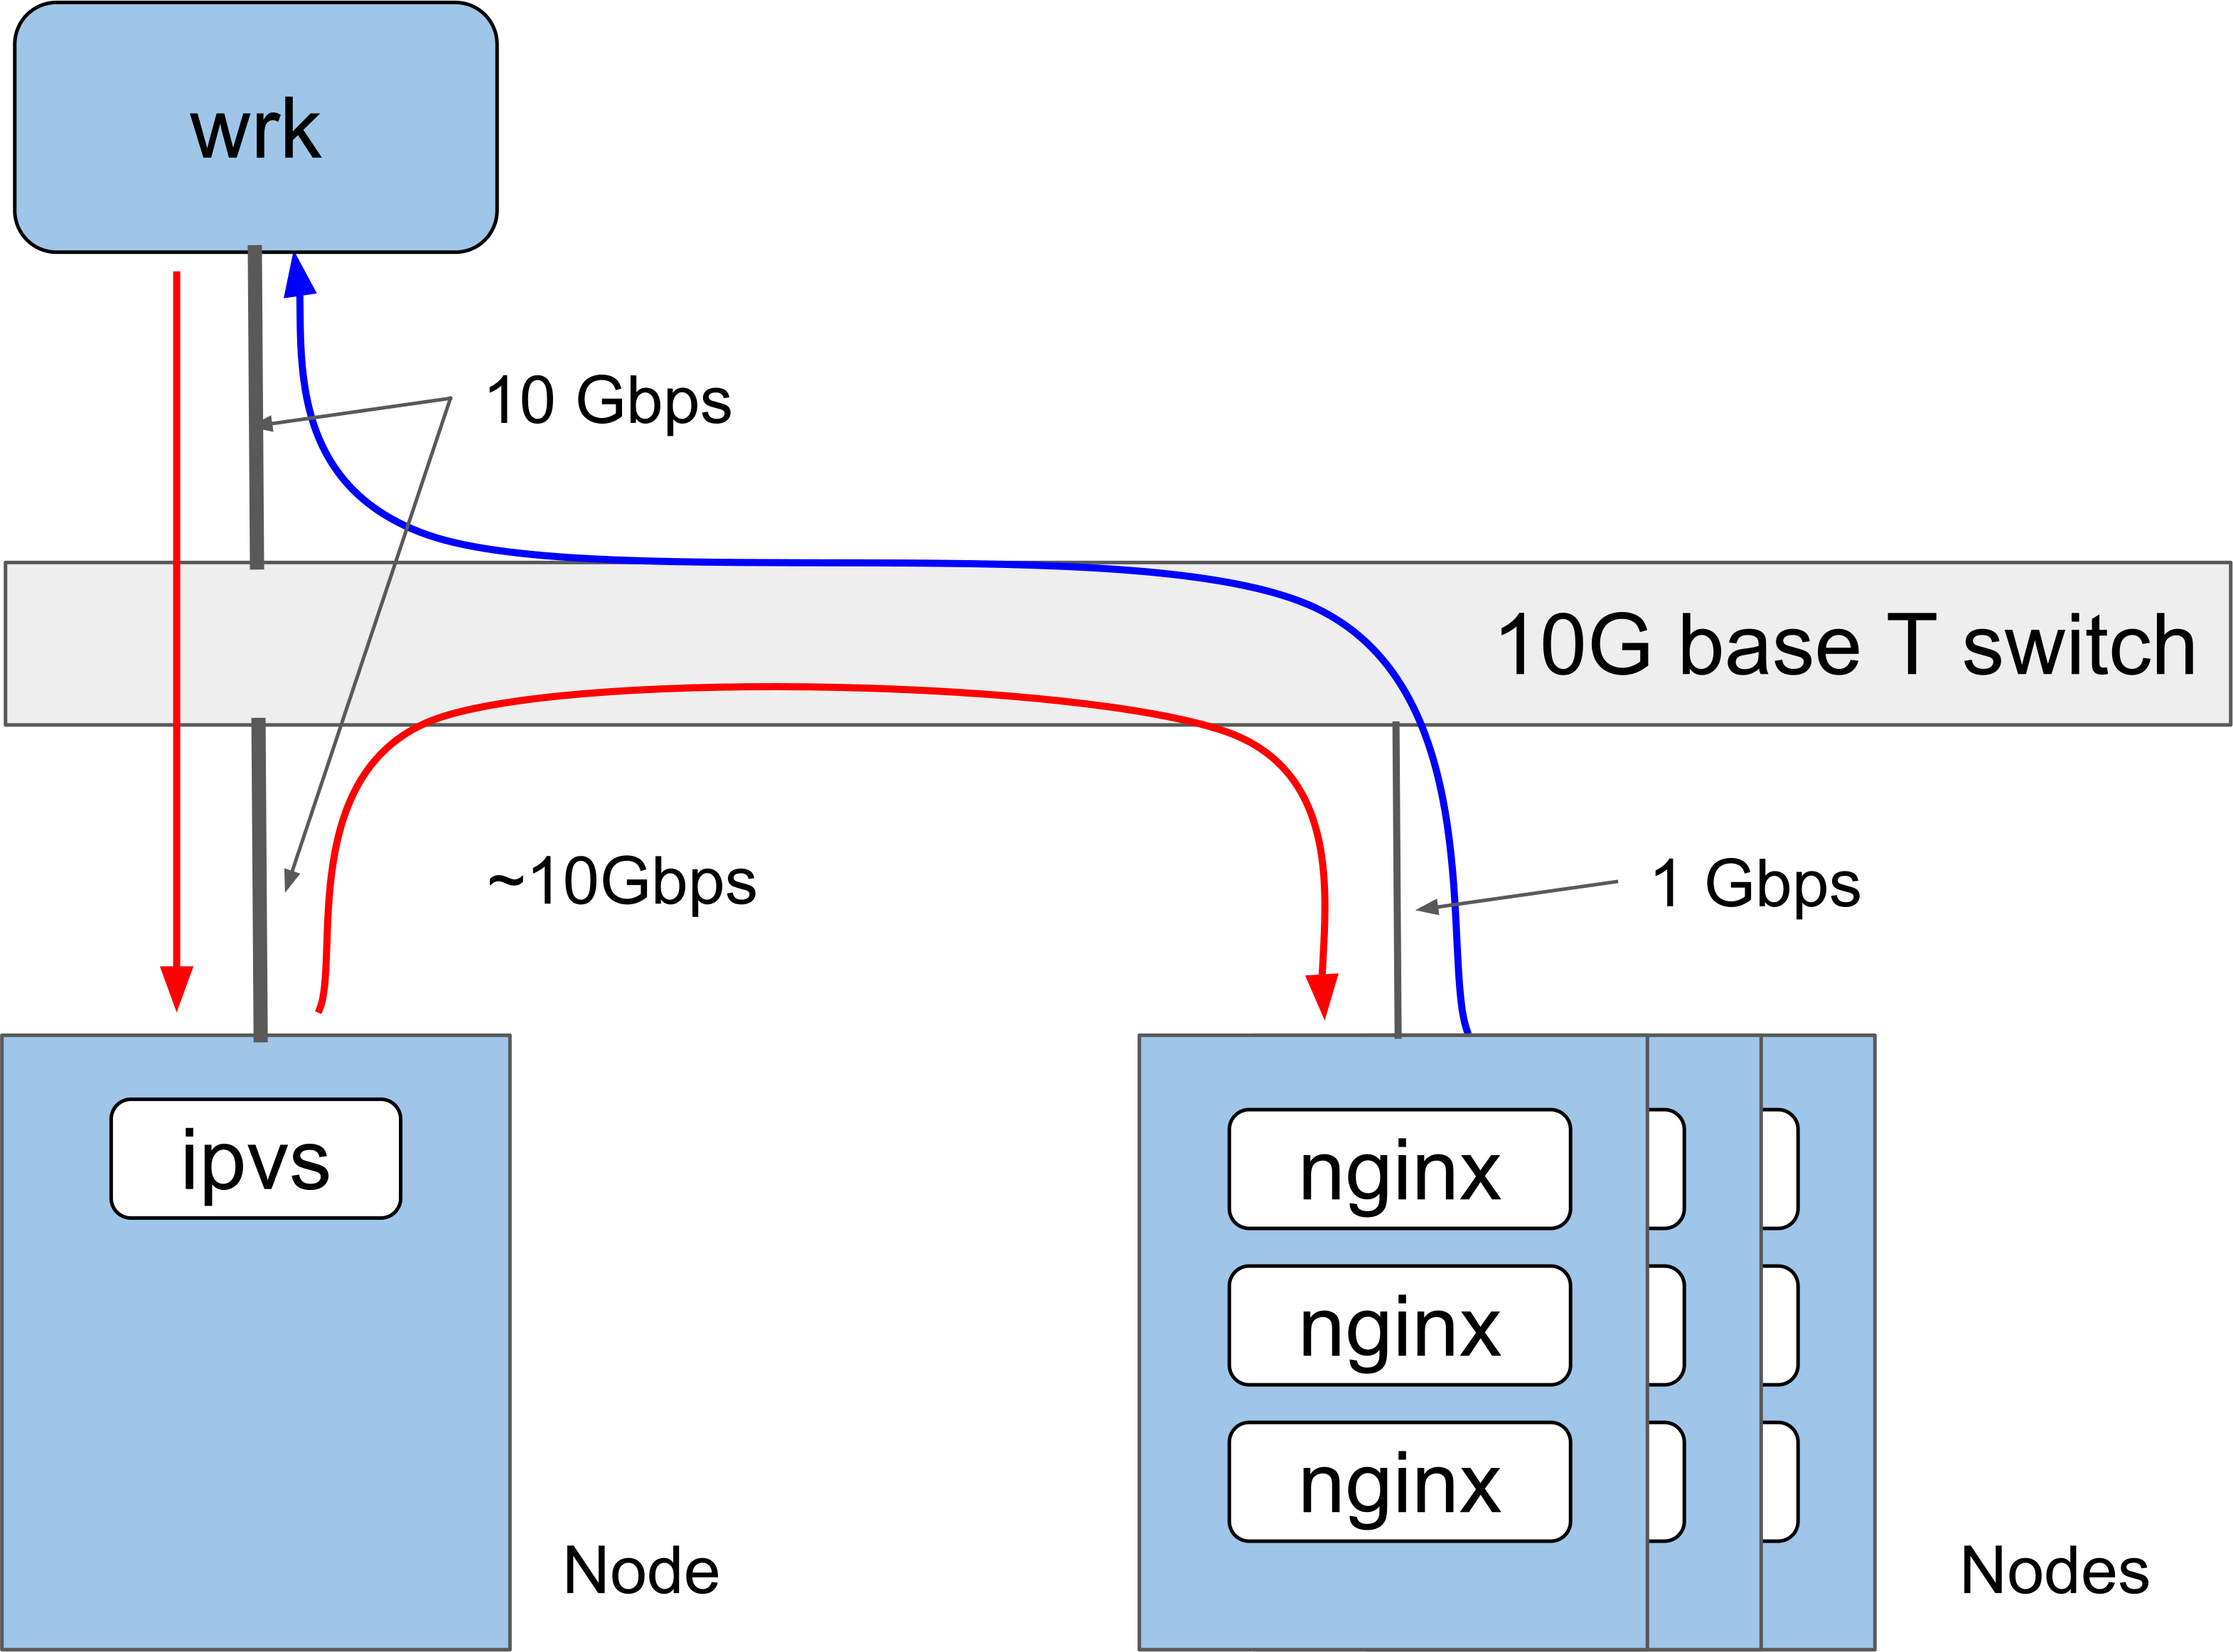
\includegraphics[width=0.8\columnwidth]{Figs/bench_10g_l3dsr}
  \caption{Physical configuration for L3DSR experiment.}
  \label{fig:bench_10g_l3dsr}
\end{figure}

\begin{figure}[t]
  \centering
  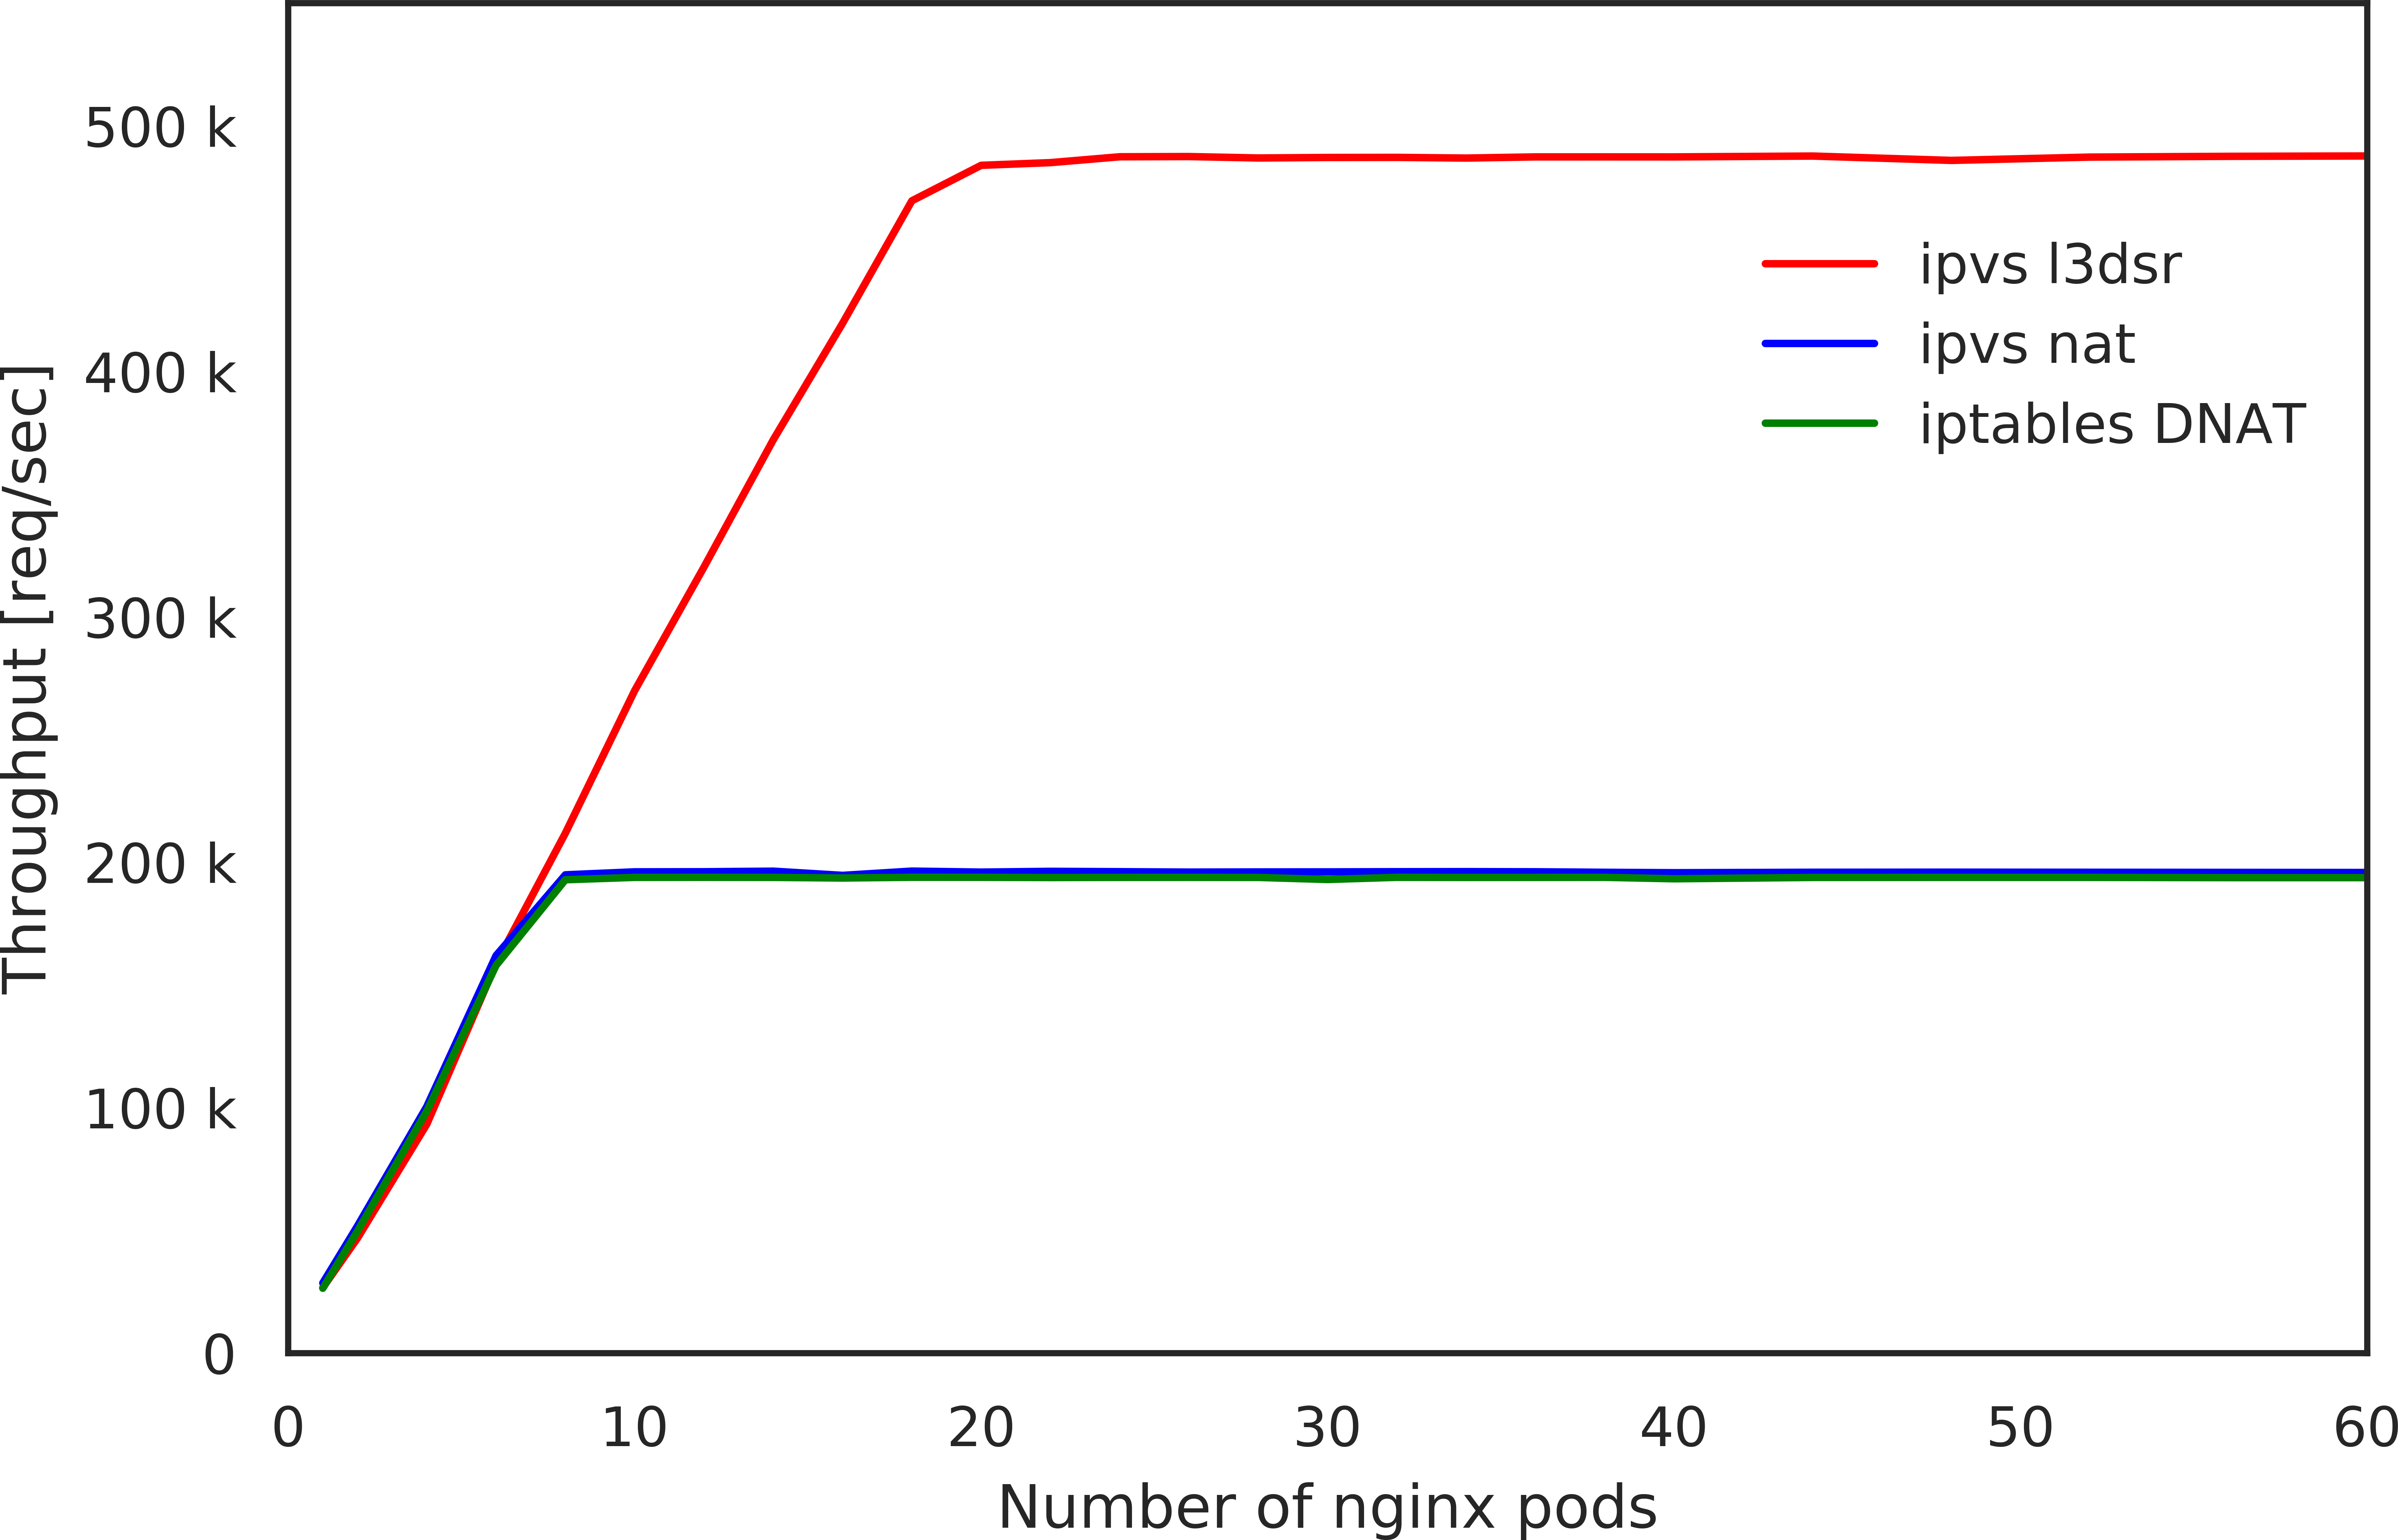
\includegraphics[width=0.8\columnwidth]{Figs/ipvs_l3dsr_1g.png}
  \caption{Throughput of ipvs l3dsr @1Gbps.}
  \label{fig:ipvs_l3dsr_1g.png}
\end{figure}

\begin{figure}[t]
  \centering
  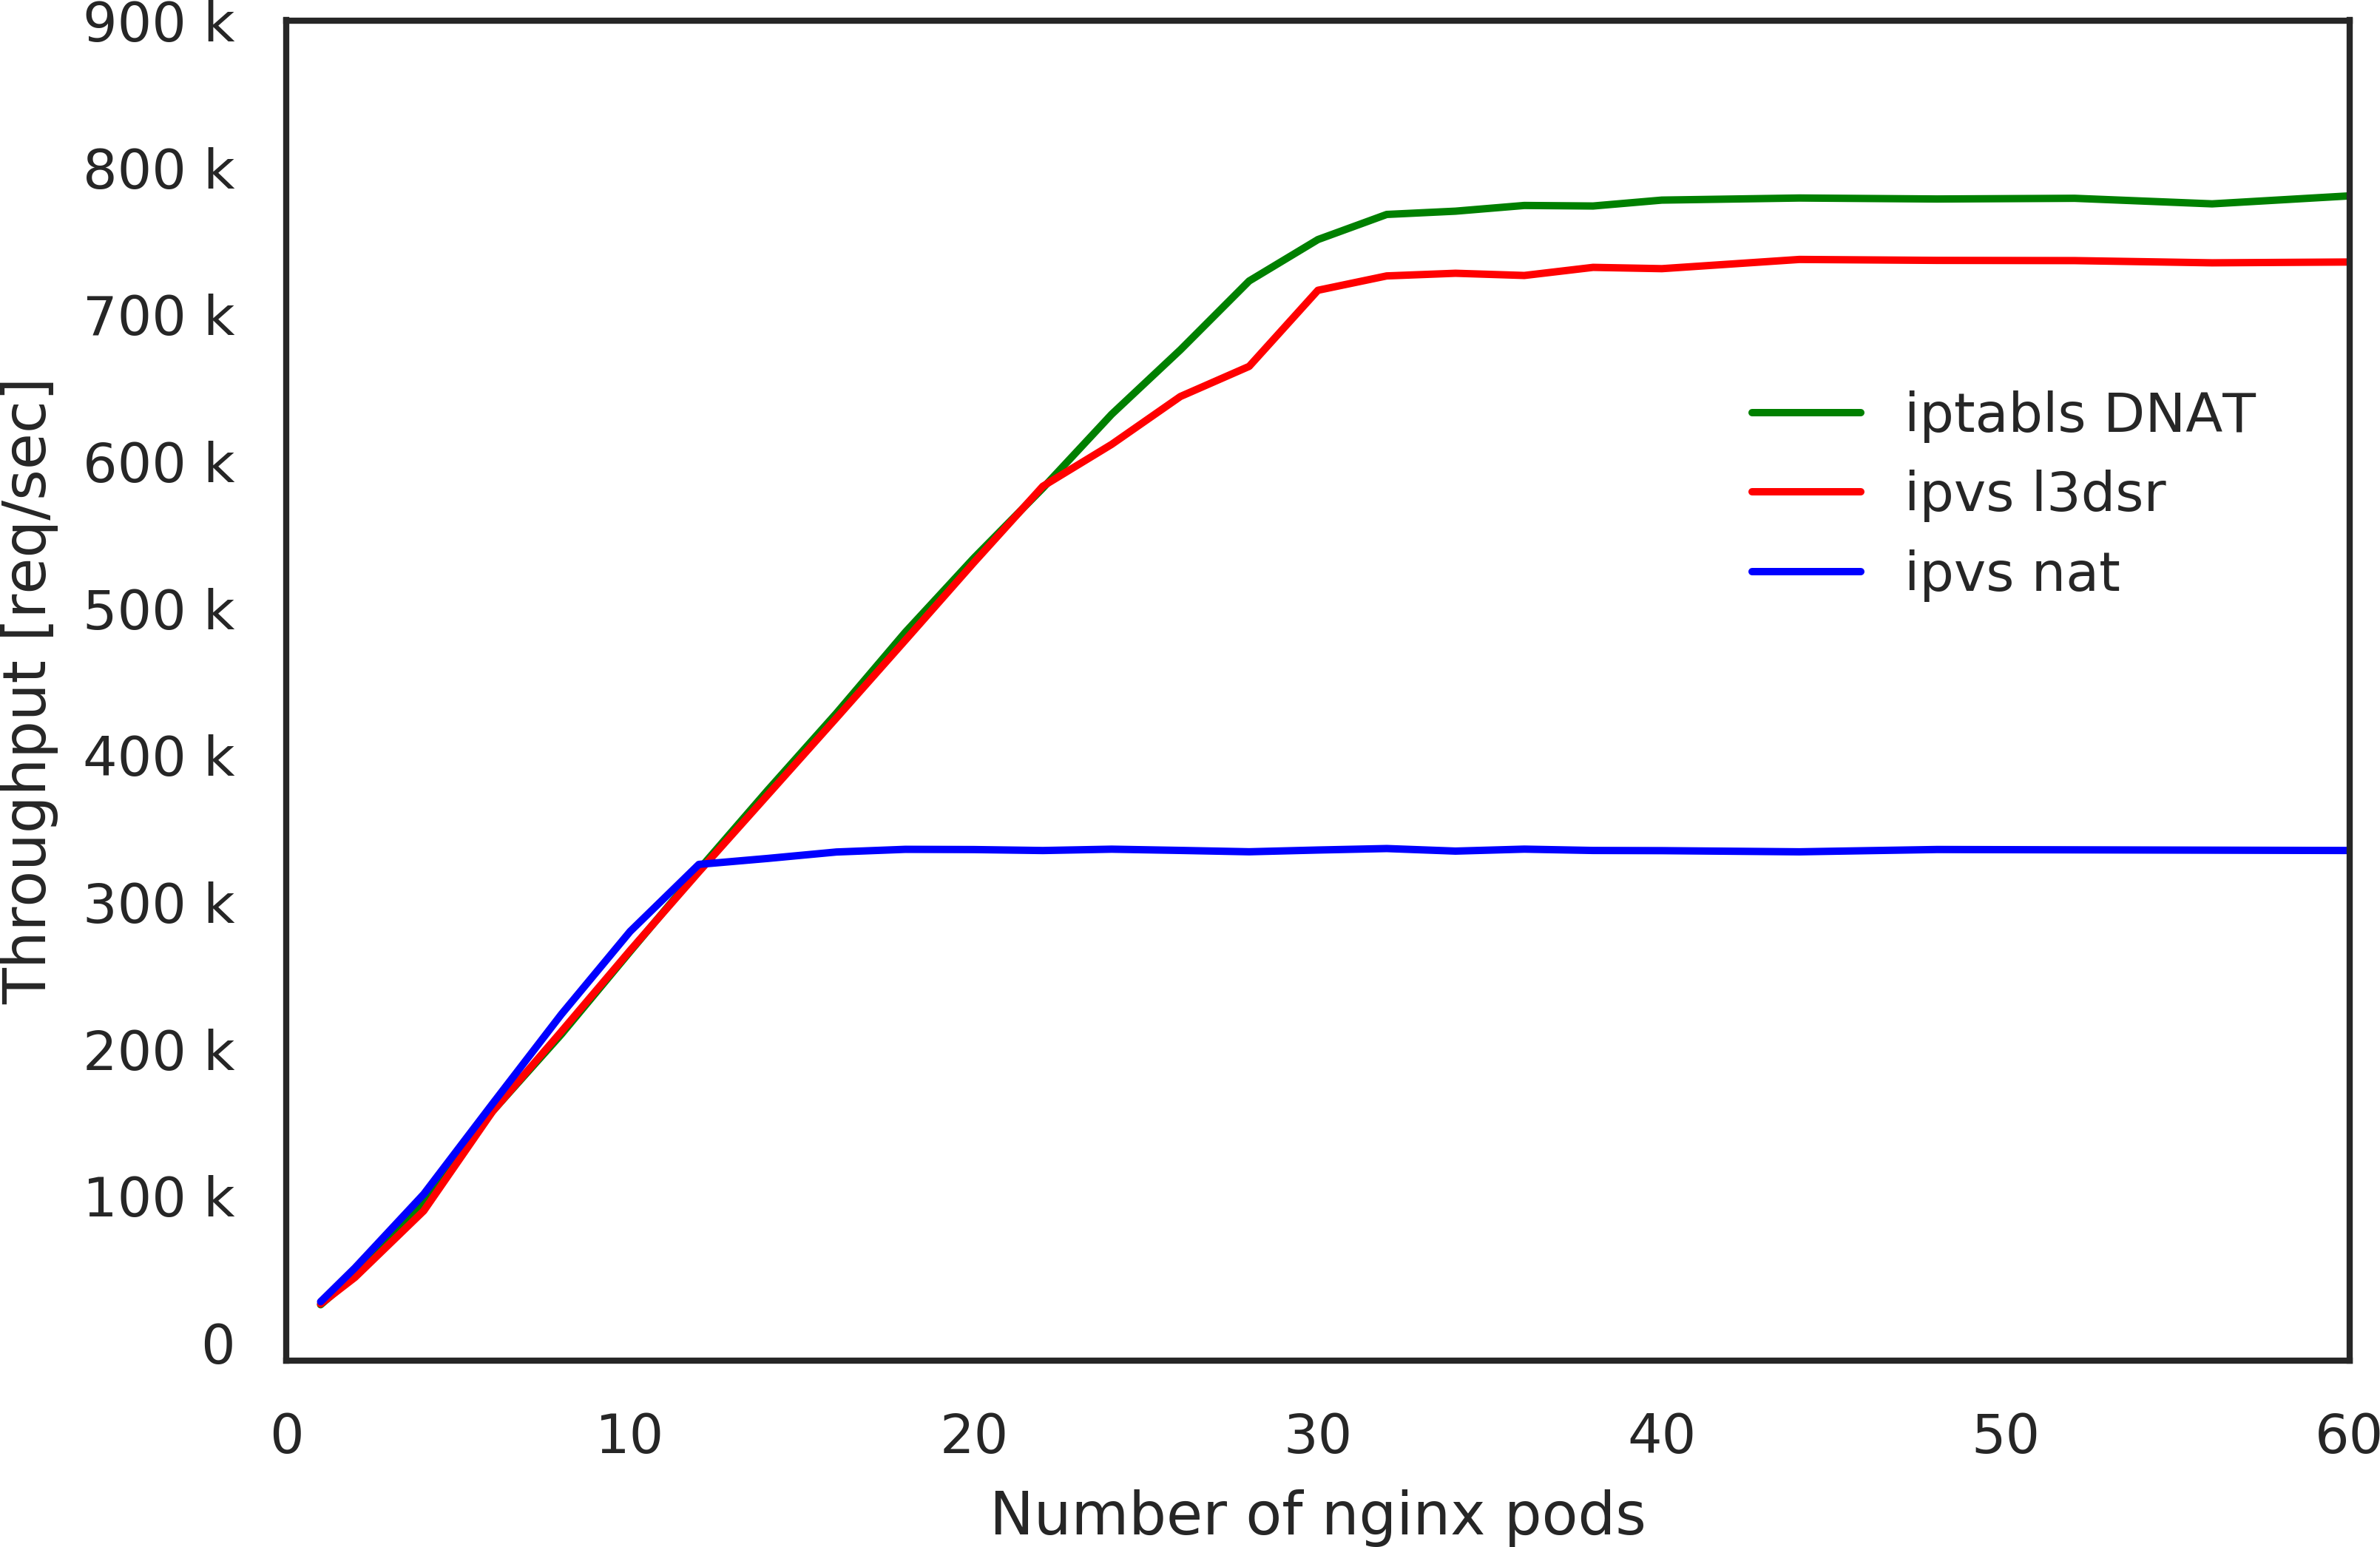
\includegraphics[width=0.8\columnwidth]{Figs/ipvs_l3dsr_10g.png}
  \caption{Throughput of ipvs l3dsr @10Gbps.}
  \label{fig:ipvs_l3dsr_10g.png}
\end{figure}

\section{Cloud experiment}

\begin{figure}[t]
  \centering
  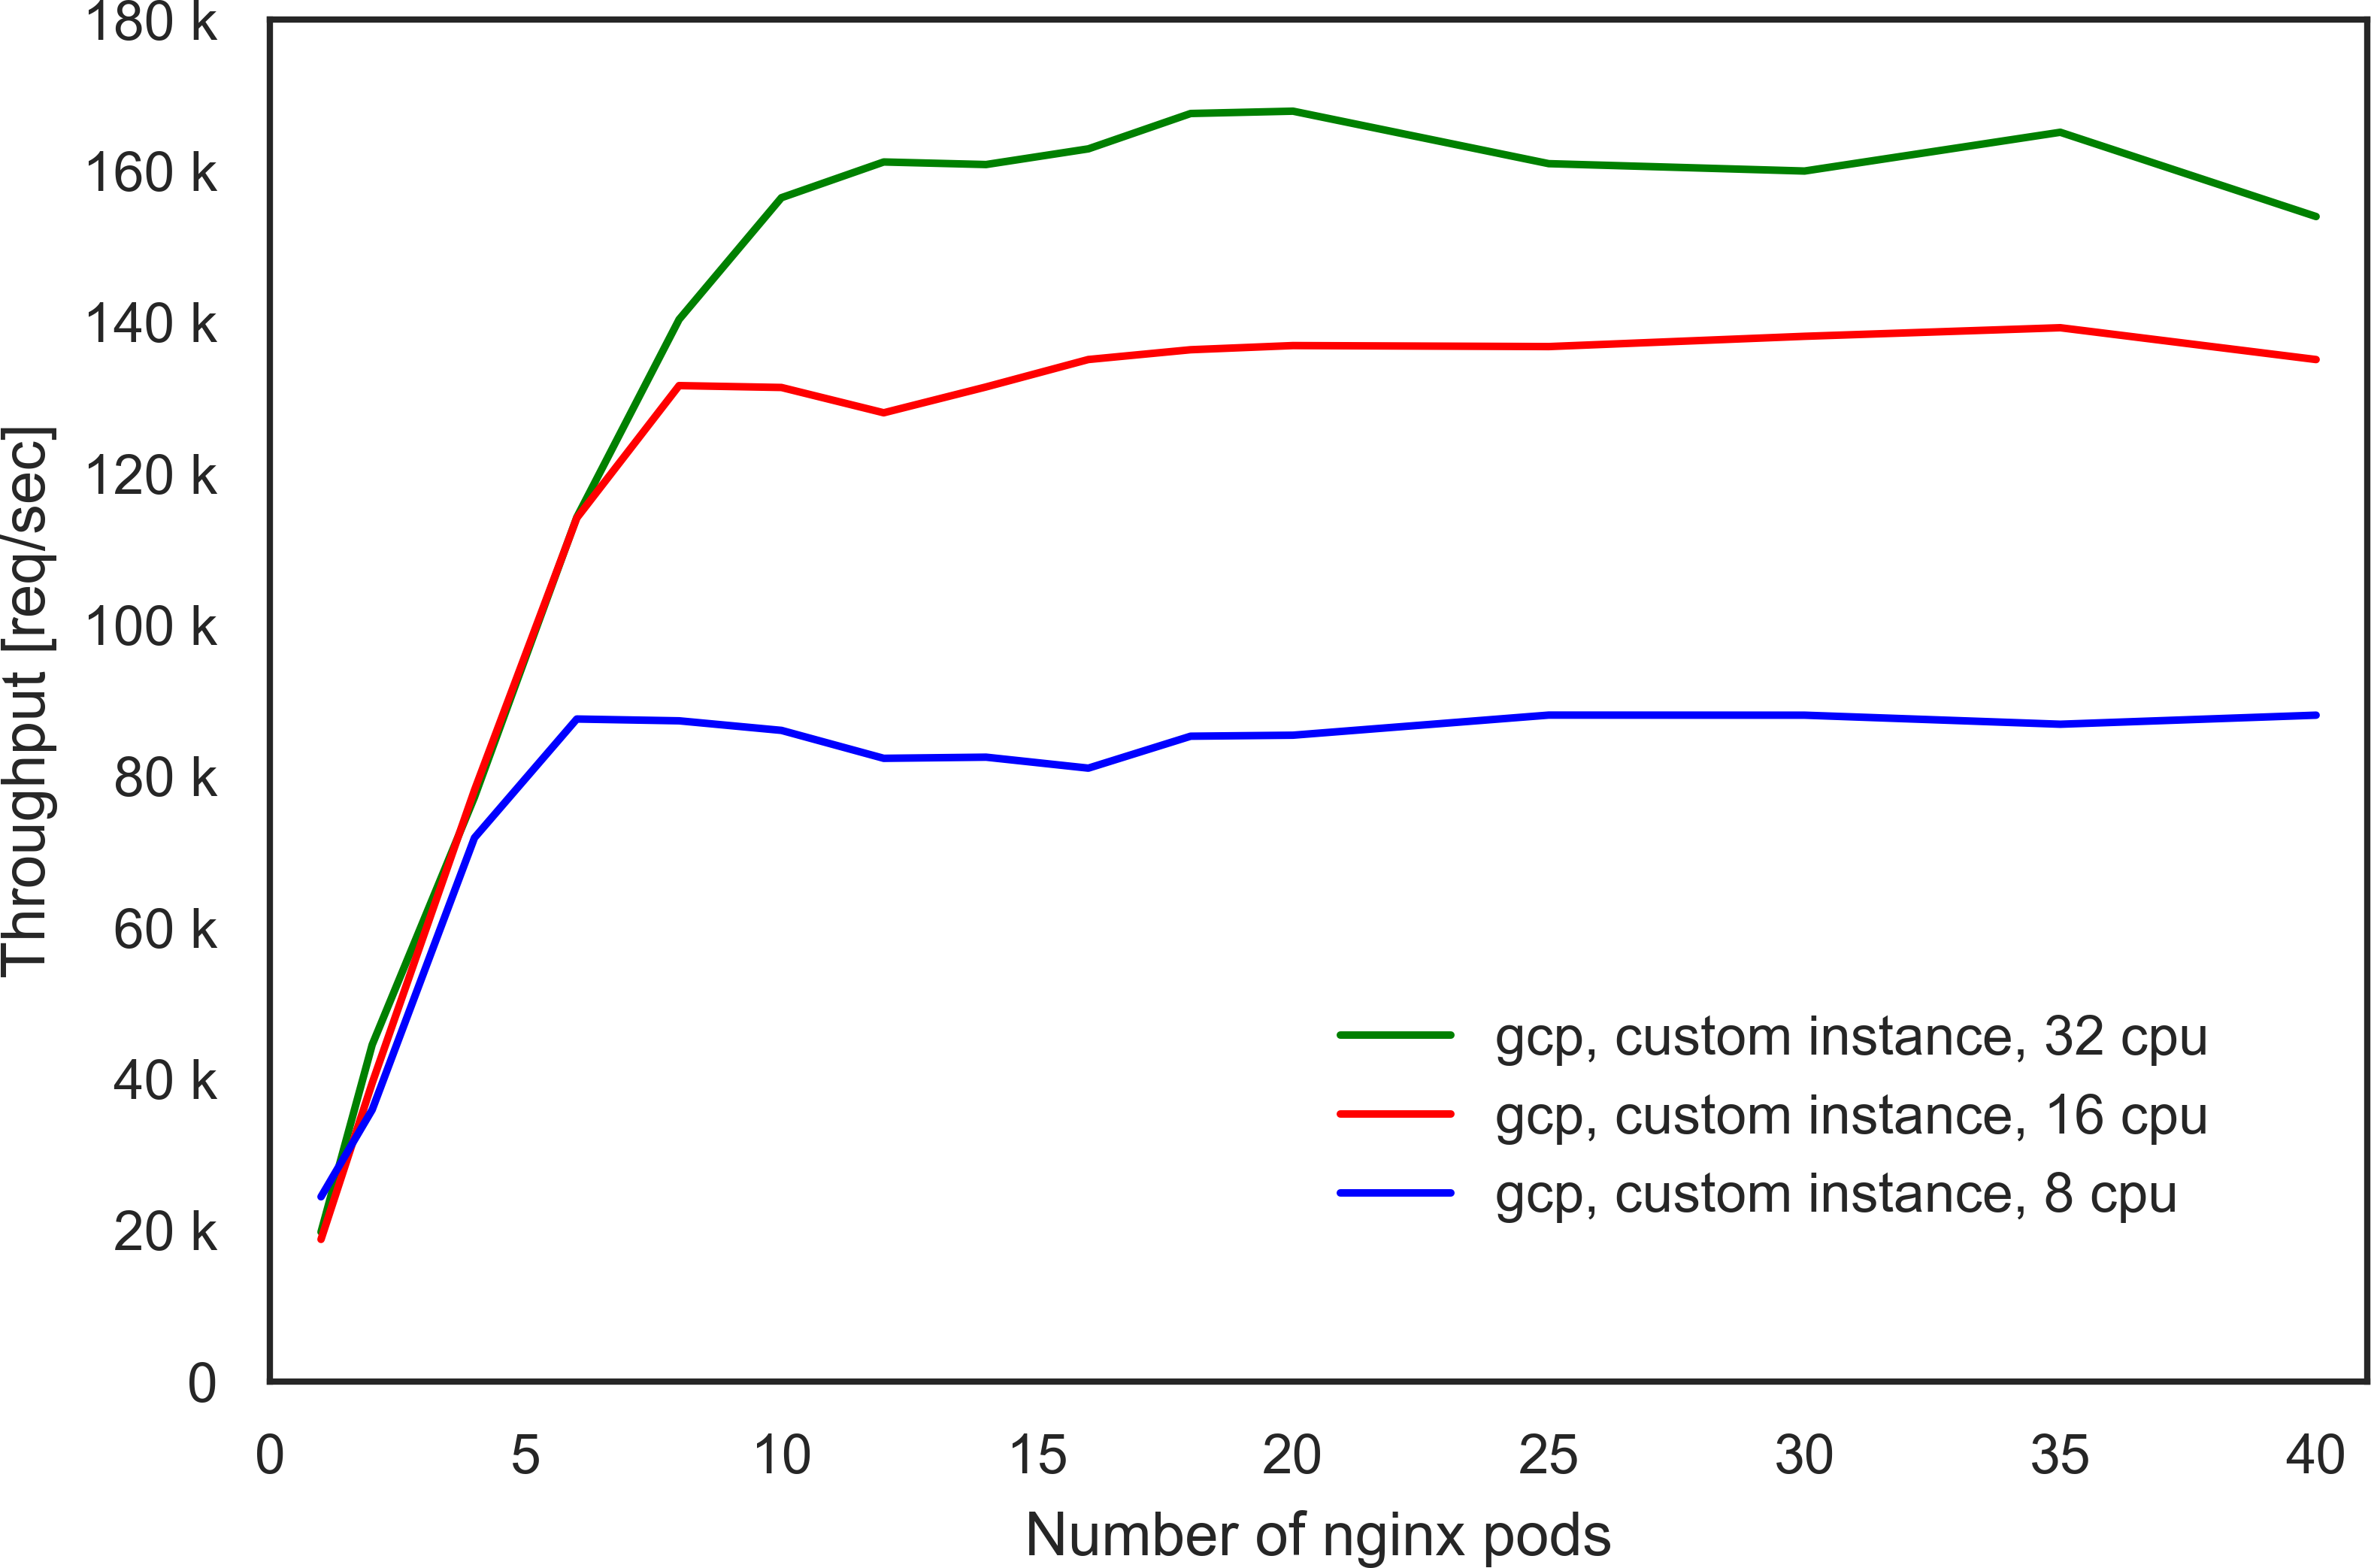
\includegraphics[width=0.8\columnwidth]{Figs/gcp_all_tp}
  \caption{GCP}
  \label{fig:gcp_all_ieice}
\end{figure}

\begin{figure}[t]
  \centering
  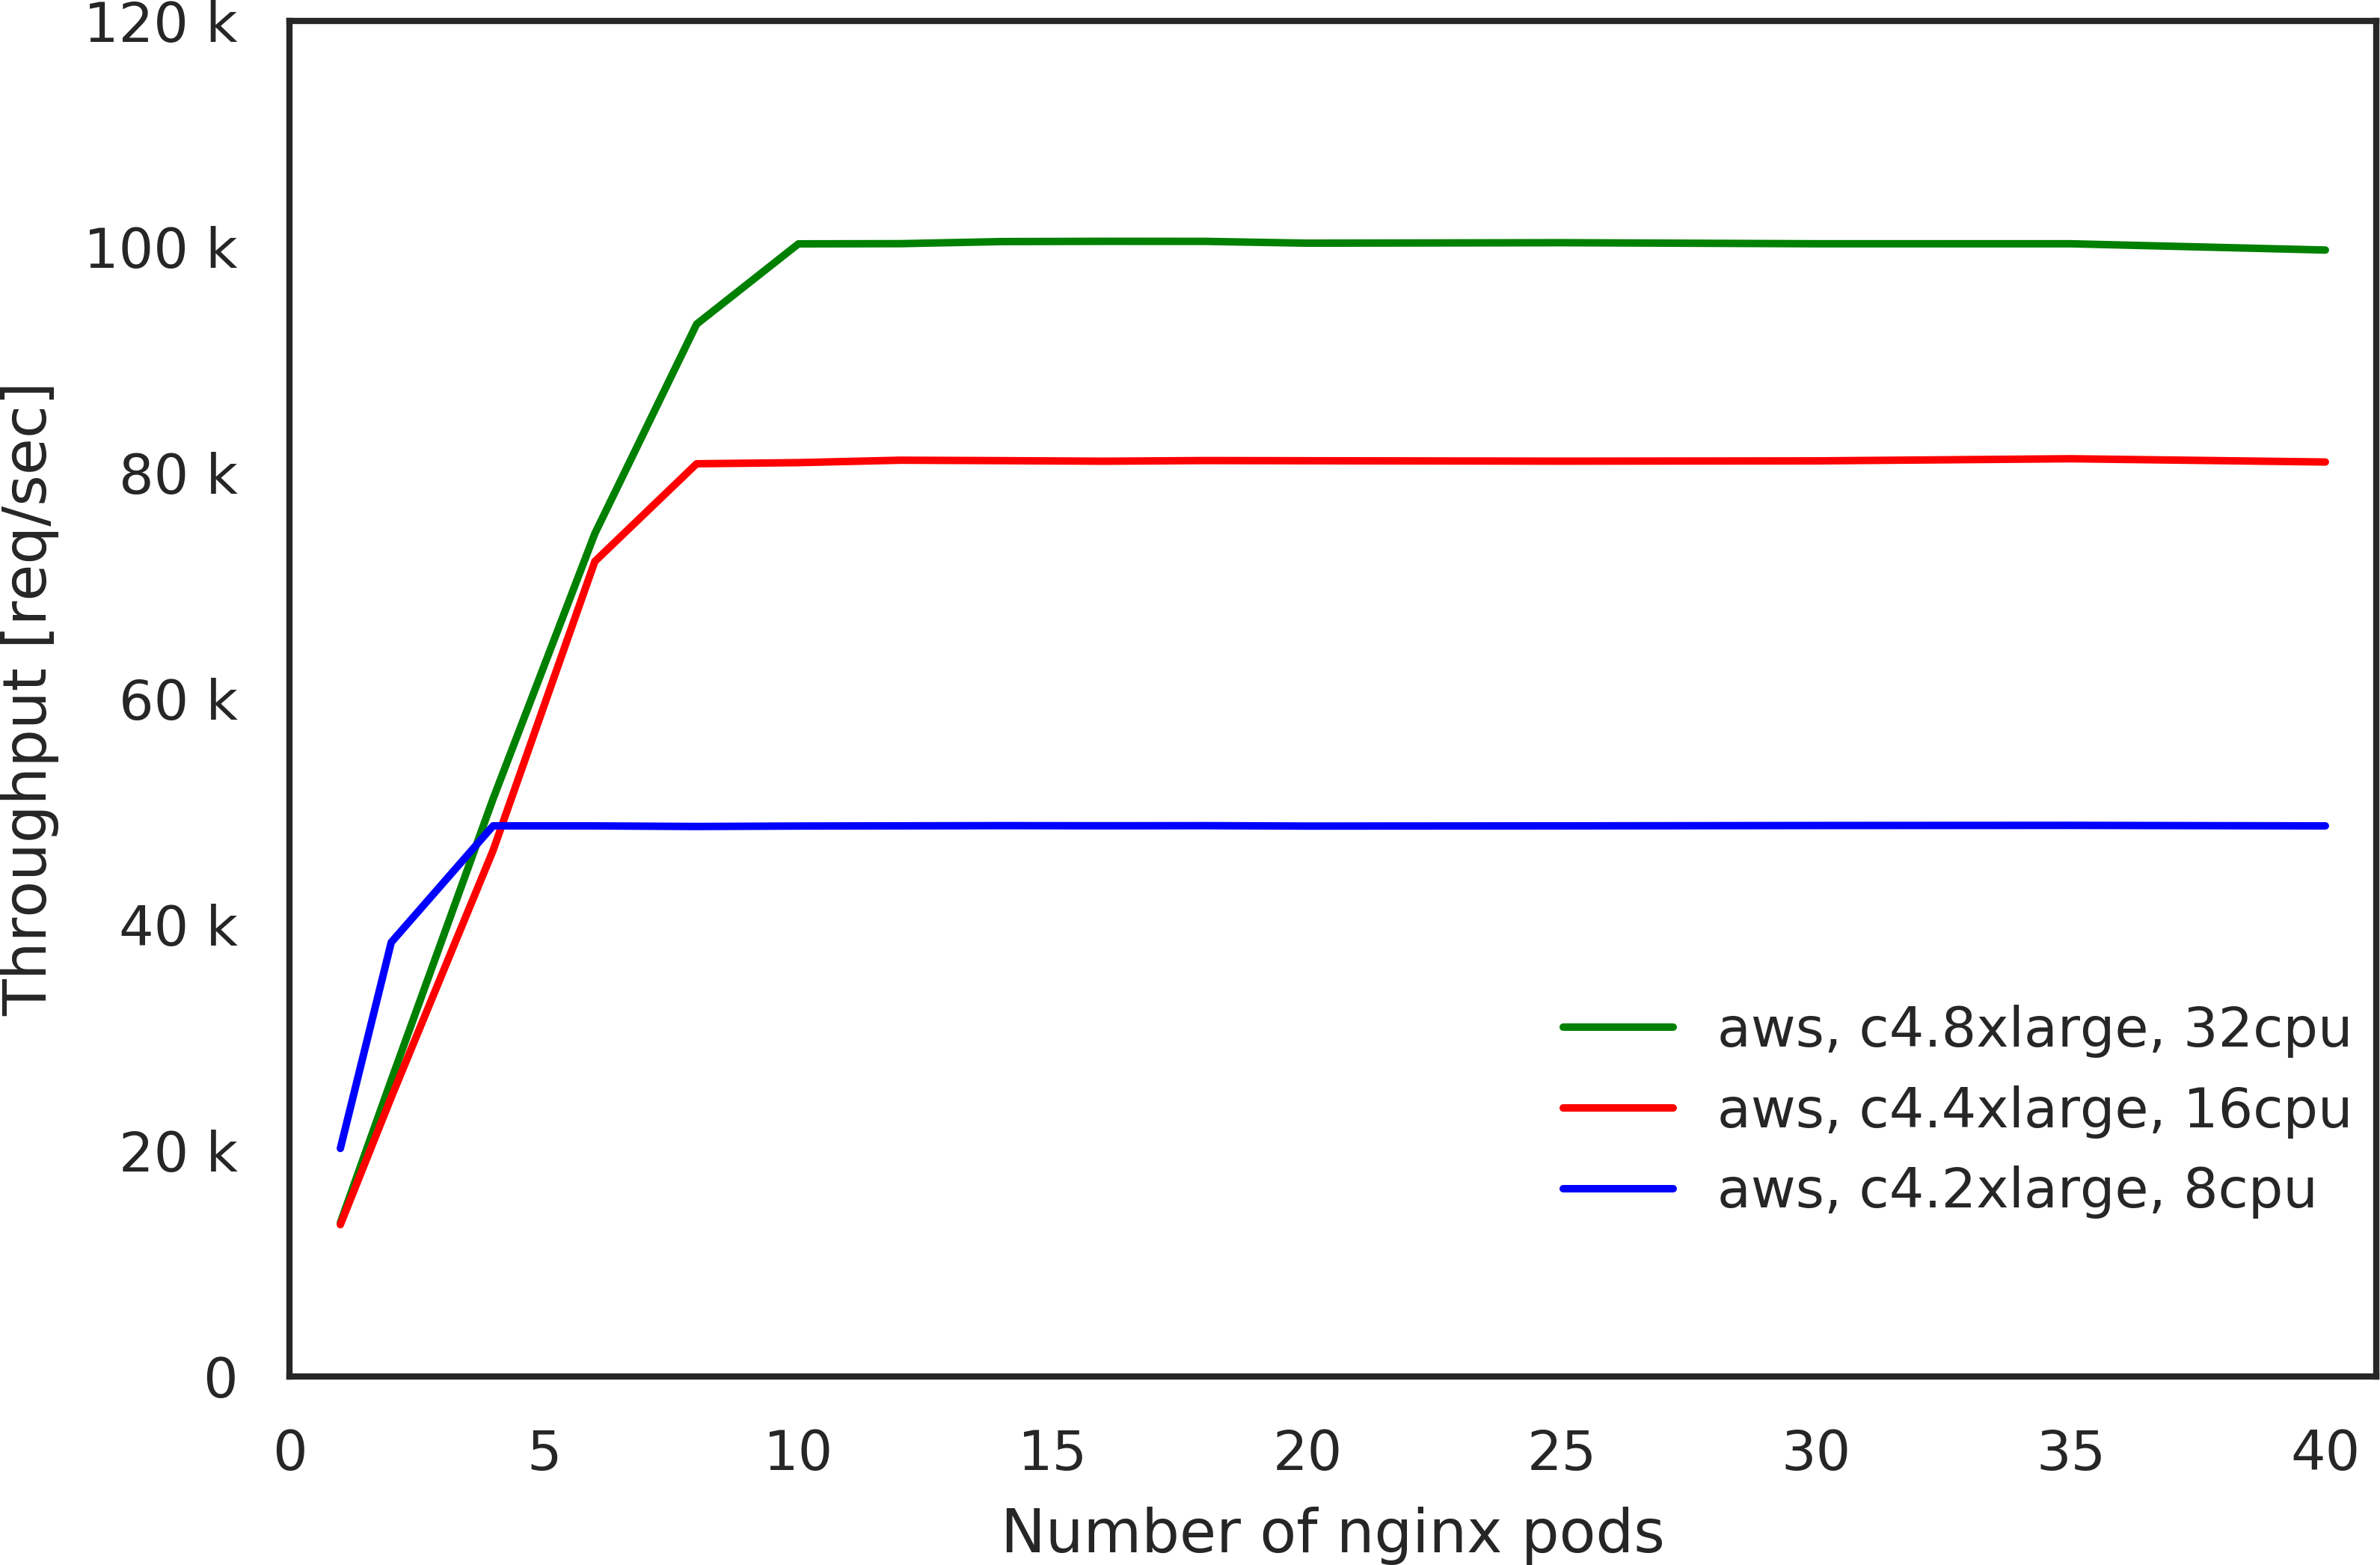
\includegraphics[width=0.8\columnwidth]{Figs/aws_c4_tp}
  \caption{AWS with Node x 6, Client x 1, Load balancer x 1. Custom instance. }
  \label{fig:aws_c4_ieice}
\end{figure}

Fig.~\ref{fig:ipvs_performance}~(\subref{fig:gcp_all_ieice}) and Fig.~\ref{fig:ipvs_performance}~(\subref{fig:aws_c4_ieice}) show the load balancer performance levels that are measured in GCP and AWS, respectively.
These are aimed to show that our proposed load balancer can be run in cloud environments and also functions properly.

Both results show similar characteristics as the experiment in an on-premise data center in Fig.~\ref{fig:ipvs_performance}~(\subref{fig:ipvs-iptables-nginx}), where throughput increased linearly to a certain saturation level that is determined by either network speed or machine specifications.
Since in the cases of cloud environments we can easily change the machine specifications, especially CPU counts, we measured throughput with several conditions of them.
From the first look of the results, since changing CPU counts changed the load balancer's throughput saturation levels, we thought VM's computation power limited the performance levels.
However, since there are cases in the cloud environment, where changing the VM types or CPU counts also changes the network bandwidth limit, a detailed analysis is further required in the future to clarify which factor limits the throughput in the cases of these cloud environments.
Still, we can say that the proposed ipvs load balancers can be run in GCP and AWS, and function properly until they reach the infrastructure limitations.

\section{Resource Consumption}

\section{Summary}



